\chapter{Early life (1936 to 1952)}

\begin{quote}
I know not who paints the pictures in memory's\break canvas; but whoever
he may be, what he is painting are pictures: by which I mean that 
he is not there with his brush simply to make a copy of all that is
happe\-ning. He takes in and leaves out according to his taste. He
makes many a big thing small and small thing big. He has no compunction 
in putting into the background that which was to the fore or\break bringing
to the front that which was behind. In short he is painting pictures, 
and not writing history.

\hfill {\small{\bf{(Rabindranath Tagore in his book ``Reminiscences")}}}
\end{quote}

I was born in 1936 in Kamuthi, a small town in Ramanatha\-puram District, 
about 80 Km south east of Madurai. It had a popula\-tion of about 10,000.\ 
There were two main streets,\break running north-south. One was called Nadar 
Bazaar and lined with shops by prosperous Nadars. The other was Muslim 
Bazaar, not so prosperous. (In my recent visit, I found the situation 
has\break reversed. The Muslims are very prosperous, while the Nadars have 
sunk.) In the north of Kamuthi, the river Gundaru ran and on its 
northern banks stood the majestic fort of Kattabomman one of the early 
chieftains who fought against the British. That area is rocky and 
elevated and hence called Kottaimedu. The Nadar houses were mostly on 
either side of the Nadar Bazaar while the Muslims lived to the west of 
their bazaar. In the\break northern part of the Muslim Bazaar were the 
Chettiars and other communities.


\begin{figure}[H]
\centering
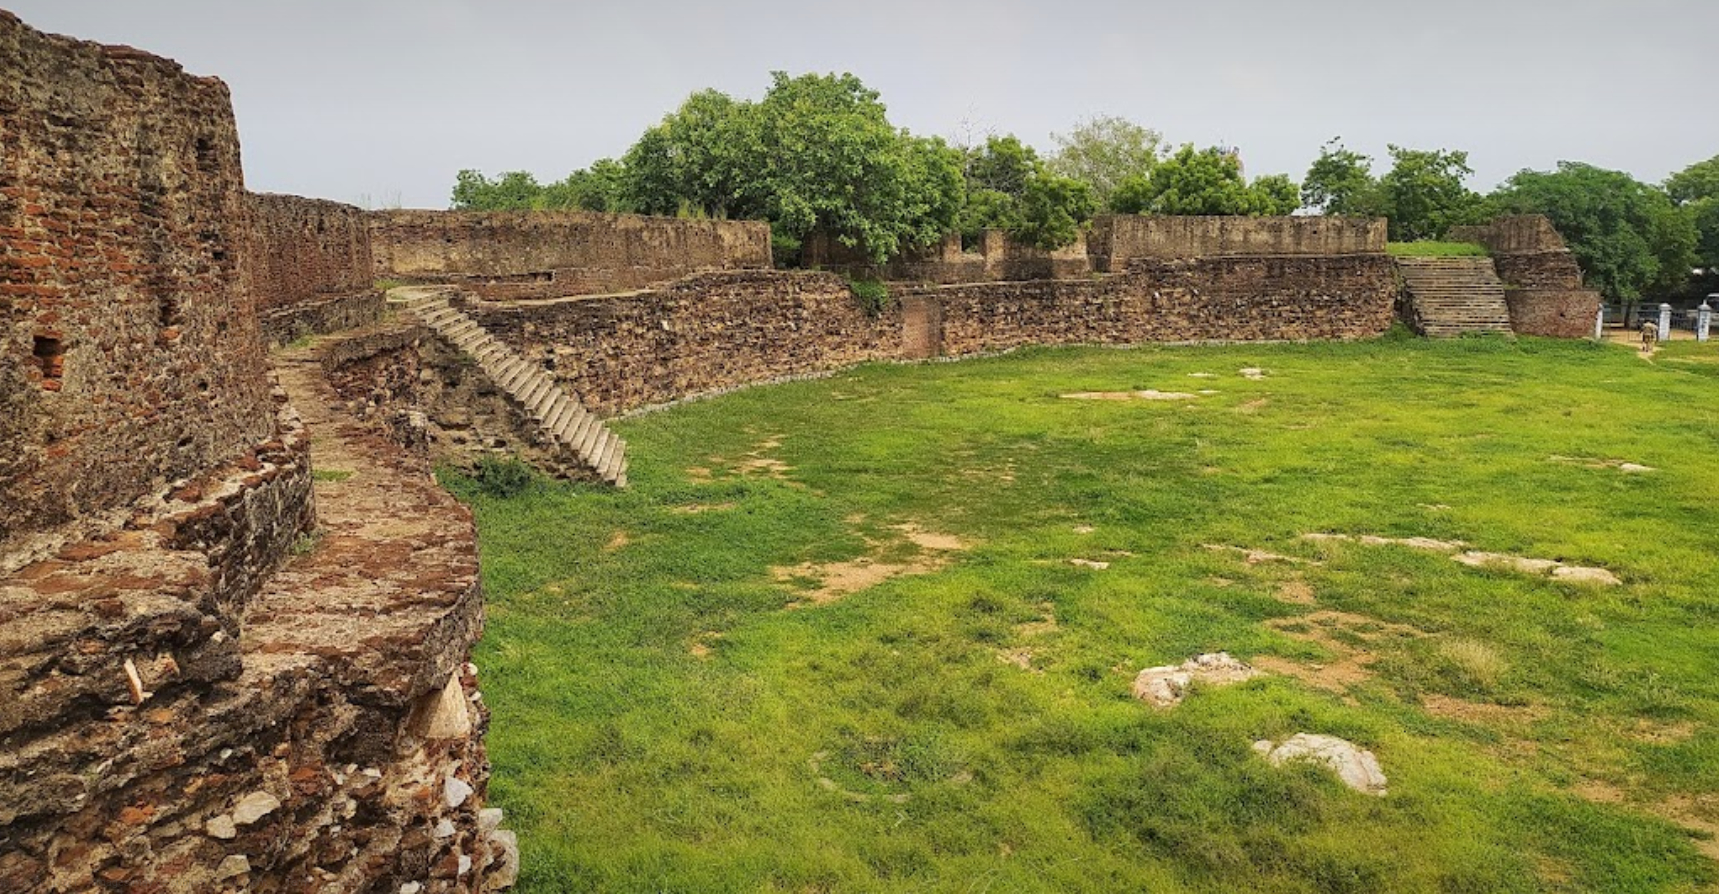
\includegraphics[width=0.9\textwidth]{images/new-images/01-Rajaji-fort.jpg}
\caption{At the top of the Kattabomman fortress}
\end{figure}

Kamuthi is in Mudukulathur Taluk which is known for\break ferocious caste 
fights. Thevars and Nadars regarded Nadars\break and Thevars respectively as 
enemies. Once before I was born, Thevars invaded Kamuthi and burnt down 
Nadar properties.\break After that every Nadar household had weapons like 
sickles and spears. That day when the plunder took place is observed 
every year by special pooja in the Muthumariamman temple. Now the fight 
is between Thevars and Harijans (Dalits) which erupts even now.

Muthuramalinga Thevar was the leader of Thevars and it was said that he 
was responsible for the caste fights. In any\break case he has been deified 
after his death. His home at Pasumpon, a village three Km north of 
Kamuthi just beyond Kottaimedu\break has become a place of worship. Every year 
on his birthday, all political leaders make a beeline to visit Pasumpon 
to pay their respects. All political parties vie with each other in 
getting the votes of Thevars who form a major vote-bank in Tamil Nadu 
politi\-cs.
 
There are two Hindu temples Muthumariamman Temple\break and Meenakshi Temple. 
There is a Roman Catholic Church and a Mosque. The Muthumariamman temple 
is in the middle of the Nadar Bazaar and it belongs to the Nadar 
community. The Meenakshi Temple belonged to the Raja of Ramnad and to 
the Thevar community. Around the Meenakshi Temple was a small Agraharam 
where the brahmin priests and teachers lived.
\smallskip

\begin{figure}[H]
\centering 
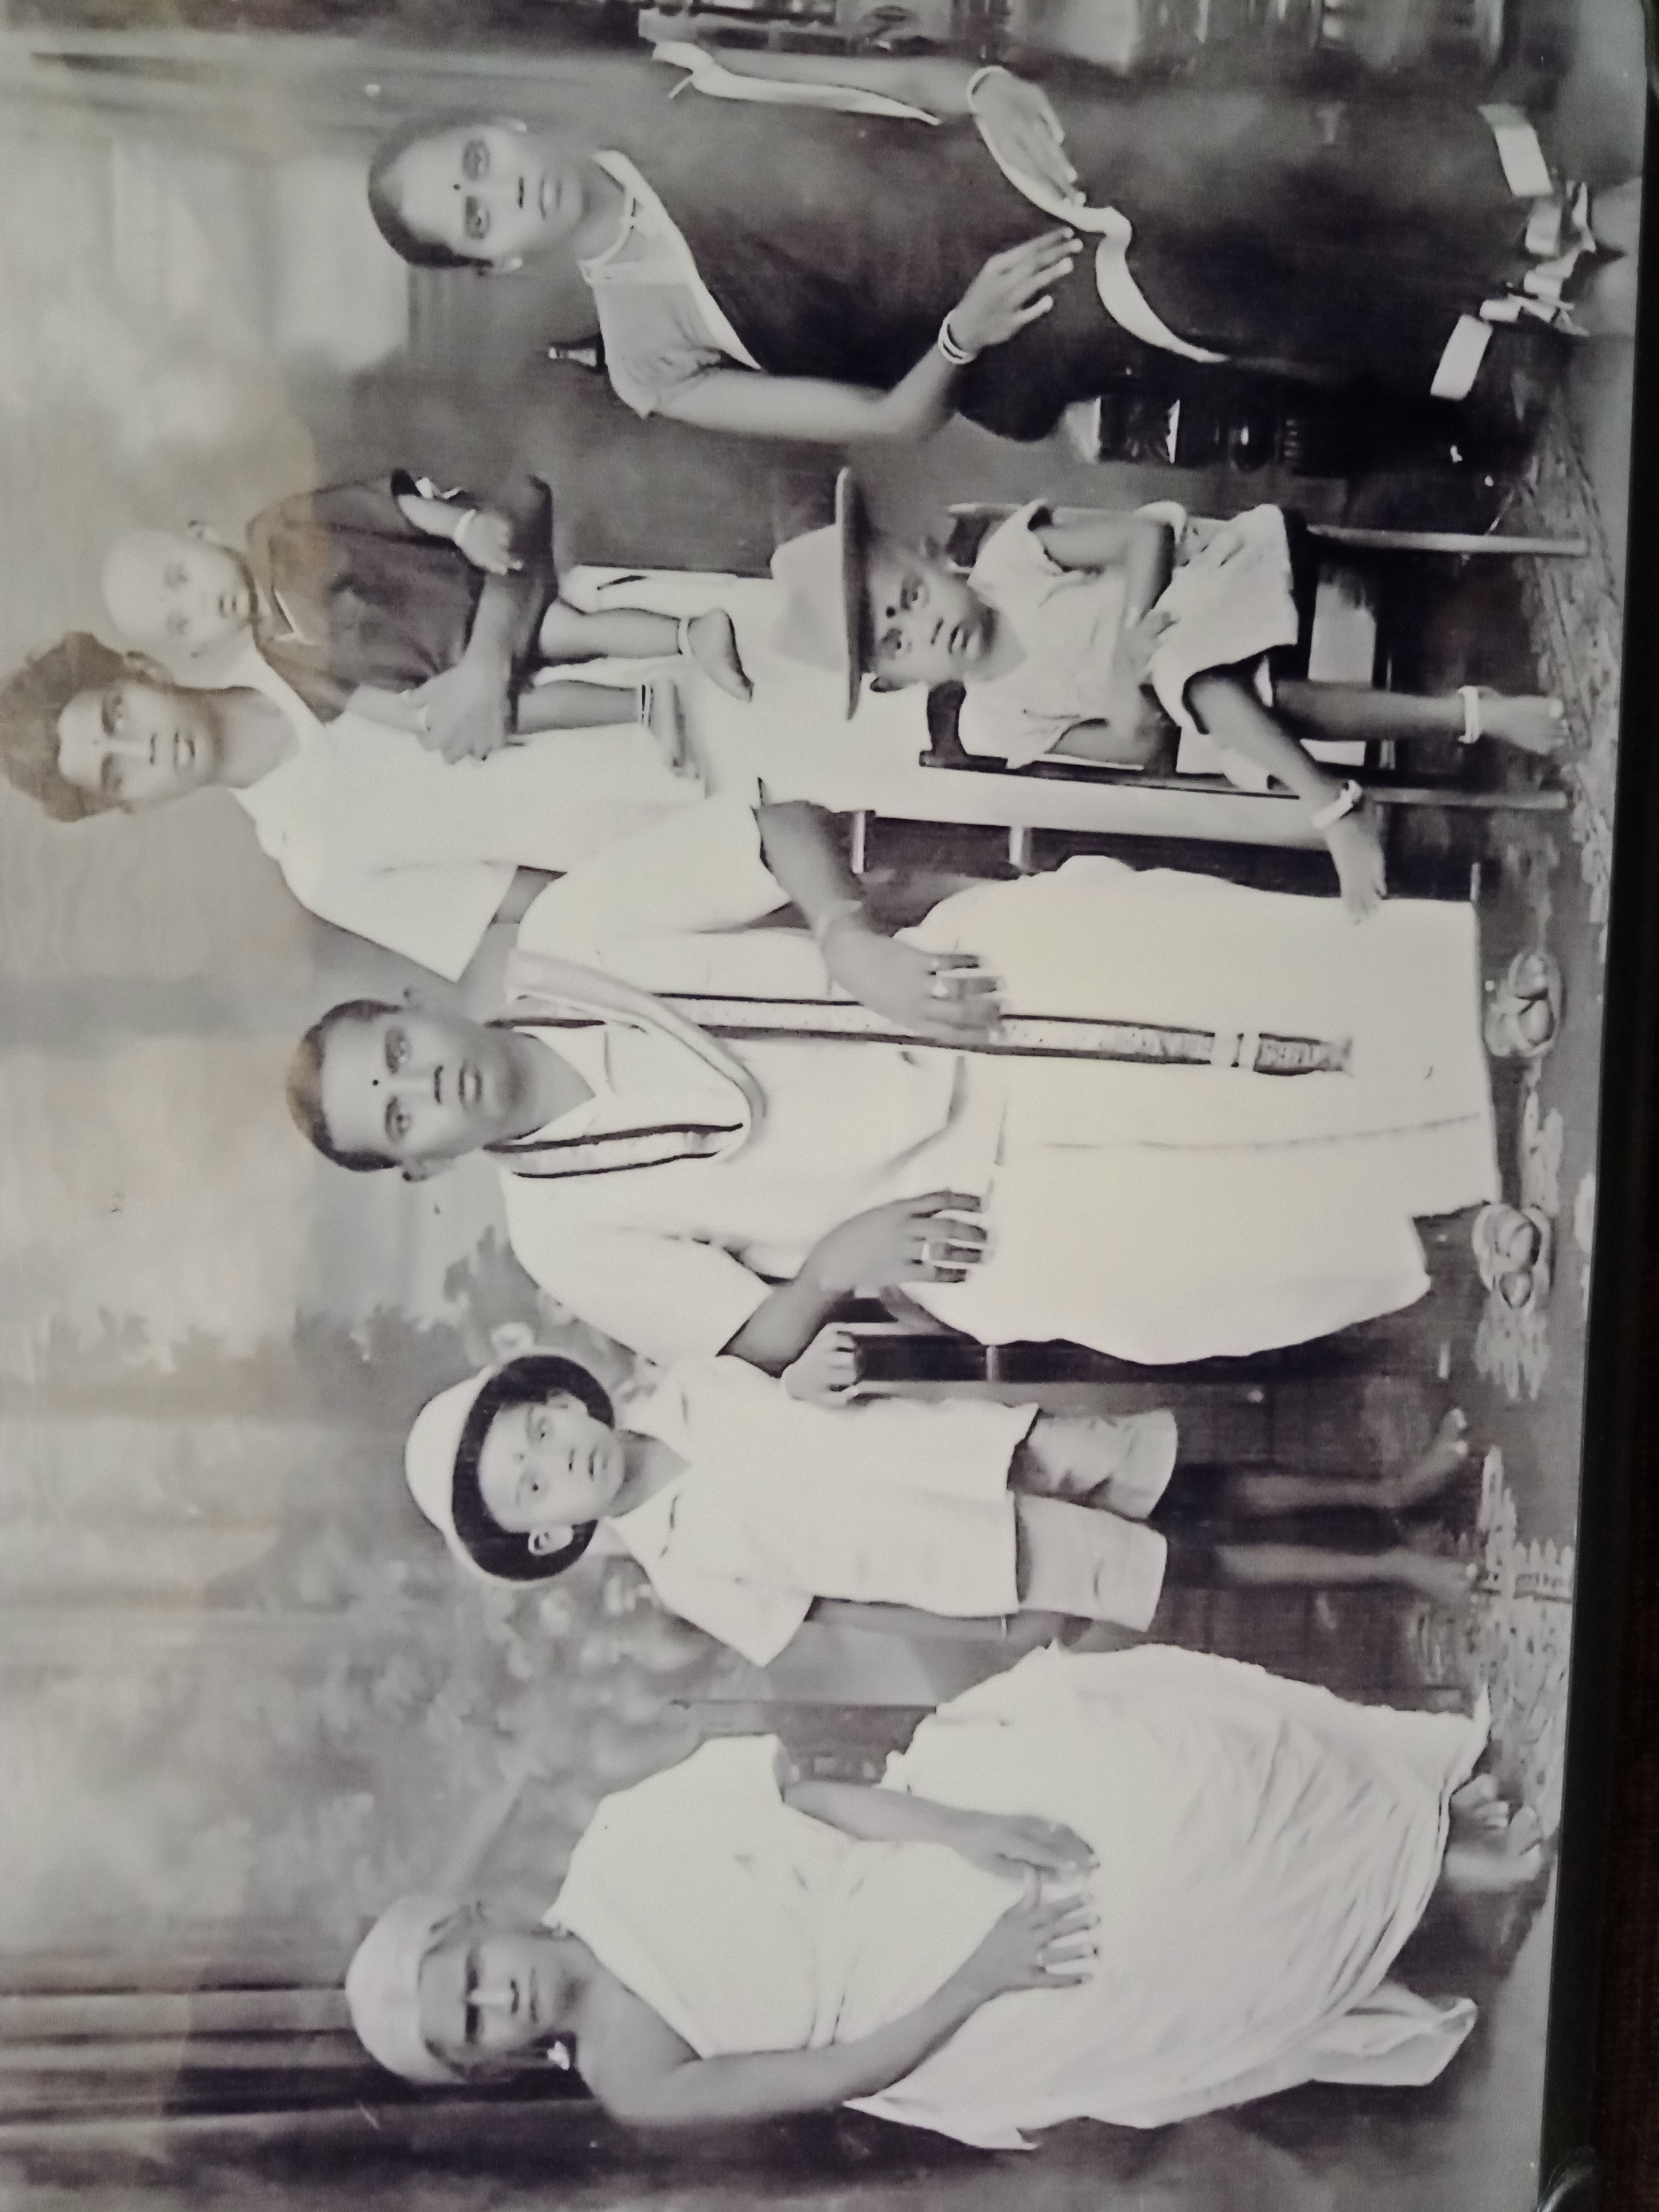
\includegraphics[angle=270, width=0.9\textwidth]{images/Rajaji-01.jpg}
\caption{\small{Circa 1942. From L to R, My grandmother, GR, my father, 
my uncle Ramalingam carrying my brother Rajaguru, my sister
Leelavathi, my mother.}}
\end{figure}

Nadars were not allowed into the Meenakshi Temple. Nadars went to the 
court on this issue, but the court said that since\break you have the 
Muthumariamman temple belonging to you, you cannot enter the Meenakshi 
Temple! Now all this is over. When I was in Kamuthi recently, I could 
enter the Temple.

My father, VR S S Guruswamy Nadar had a shop selling metal vessels. My 
mother was Ekkimuthammal. I was the first born and had four brothers and 
five sisters, one of the sisters died as an infant.

My father's shop did well and so our family was reasonably well- 
provided, but later my father's earnings in the shop was not enough to 
provide for such a large family.

My father's father, whom I never saw, was Sivagurunatha Nadar. His 
father was perhaps Subramania Nadar and his\break father was Veerabhadra 
Nadar. So my father's initials start from VR (Veera), then S (Subra), 
and S (Siva). This is how Nadars were generally named. If I were to 
follow this practice, my name would be VR S S G Rajasekara Nadar! 
Although my grand father was not alive when I was born, I was lucky to 
see my grandmother. She passed away when I was in the elementary school.
\vskip 1pt
My father's family was not well-to-do. My father studied only up to 
second standard. In fact I heard that the family was so poor that my 
father made whistles out of palm leaves and sold them to children!
\vskip 1pt
He went to Rangoon and worked as a shop assistant. Those days Indians 
went to Burma or Malaya just as now they go to USA or Middle East. After 
earning enough money he returned and got his three sisters married off. 
Then he married my mother in 1934. As I already said, he did very well 
through the vessel shop.
\vskip 1pt
My mother's father was MR Perumal Nadar. He went to\break Penang in Malaya and 
did very well. He owned his own shop there. He took my mother to Penang 
for some time. So both my father and mother are foreign-returned!
\vskip 1pt
As ill luck would have it, during the Japanese occupation\break at the time of 
the Second World War, my grand father had to convert all his money into 
Japanese currency which became\break worthless after the war. He brought all 
these currency notes and distributed them among children; we used to 
play with them!
\vskip 1pt

But his return to India was an interesting story. For many years during 
the war we did not have any contact with him. It was even thought that 
he was dead. I remember I was persuaded to write a nice letter to him by 
my uncle Ramalingam (my\break mother's younger brother) for which of course 
there was no\break reply.
\vskip 1pt

Around the year 1947, my father wanted to take our whole family on a 
pilgrimage to a small town called Yeral. We were waiting for our bus at 
the bus stand. Imagine our surprise, when Perumal Nadar got down from 
the bus!

Perumal Nadar was a very interesting personality. He used to take me to 
the river-side for long walks and advised me to pluck the herbs there 
and eat them. He was also philosophically oriented and gave me many 
books to read.
\vskip 1pt
In my younger days my uncle Ramalingam who was looking after our shop 
took care of me also, like taking me to the well (called Nandavanam) for 
bath, when my father was not there. In fact most of the time I was with 
him in the shop.
\vskip 1pt
There were two deaths which affected me very much in\break my childhood.\ My 
baby sister Kanthimathi and my aunt\break (Ramalingam's young wife). The 
latter died while giving birth to her first son. She was very fond of 
me.
\vskip 1pt
I had three aunts (my father's sisters) Mookkammal,\break Thenammal and 
Sornammal who lived in another small village, Kokkarankottai. Thenammal 
lived in Aruppukkottai, another town. Mookkammal lived in Kamuthi. Her 
husband died\break before I was born. She liked me very much and I visited her 
small hut often. She was very poor, but always gave me something to eat. 
Once she could give me only rice mixed with brinjal cooked in oil. It 
was so tasty that even now I like brinjal cooked that way. My father's 
elder brother Rangaswamy Nadar had a vessel shop in a neighboring town 
Abiramam, but did not do well.
\vskip 1pt
There was a Sankara Mutt in Kamuthi. A few Nadars and maybe some from 
other communities belonged to the\break Mutt. My aunt Mookkammal also belonged 
to it. They were all vegetarians. Once a year there was a pooja and 
meals were served. My aunt took me there.
\vskip 1pt
Another person I liked was my maternal grand mother's\break sister Meenammal. 
Tragically she had lost her husband and\break son some time ago. She liked me 
very much and as a child I remem\-ber to have spent much time with her in 
her humble hut. She was very poor and eked out a living by selling the 
milk from one or two buffaloes that she kept. She used to carry me on 
her rounds selling the milk.

Meenammal used to go for groundnut-picking in the\break fields north of 
Kamuthi and she often took me there. The plants had been plucked along 
with the roots. We had to pluck the groundnuts from the roots. At the 
end of the day, one-sixth of what we plucked was our wage. We used to 
roast some of the groundnuts on open fire there itself and they were 
very tasty to eat. My father would not allow me to go, so I went only 
when he was away in Madurai!

My father along with another Nadar ran a Cinema Theater. I still 
remember my father taking me on the back seat of a\break bicycle to watch the 
films. But I heard that my father lost a lot of money since the other 
person cheated him. I also heard that the only film that ran well and so 
earned some money for him was ``Rajasekaran" and that is why my father 
named me that!

The very first film that I understood was Nandakumar. My uncle 
Ramalingam took me for it.\ TR Mahalingam acted as\break young Krishna and I 
liked it. Another film that I liked and still remember is Laila Majnu. 
There were two versions: one with Nageswara Rao and Bhanumathi with 
Gantasala's songs and the other with TR Mahalingam. Much later when I 
was in American\- College, Madurai, I saw Devadas (with Nageswara Rao and\break 
Savitri) and I liked it very much.

The other films that I liked were Bhaktha Meera (MS Subbu\-lakshmi), Shakunthalai (MSS), Savitri (MSS), Sivakavi (MK\break Thiagaraja Bhagavathar), Thiruneelakandar (MKT), Haridas\break (MKT), Chakradhari (V Nagiah). The other singing stars that I liked were PU Cinnappa, TR Mahalingam and KB Sunda\-rambal.

There was not much industry in Kamuthi. But I can mention a few things 
of interest. RM T S Soundara Pandian's family was well-to-do among the 
Nadar families and they had earned their money by leather business from 
the time of RM T S S's father Senthilkumar Nadar. They bought the skins 
of the slaughtered goats, treated them and after further treatment in 
their factories in Dindigul and Trichy, sold them. Some were even 
exported abroad.

RM T S S was an important Congress leader in the district and knew 
Kamaraj who visited Kamuthi a few times. He was elected as the President 
of the Panchayat Board. My wife is his daughter. He named her Suthandra 
Devi (Goddess of Liberty) since she was born just after India got 
independance. He passed away during the election propaganda when he was 
talking in support of the Congress candidate.

Another prosperous family in Kamuthi was the family of\break PNSP Palanichamy 
Nadar who made their money by making\break snuff from tobacco. Their firm was 
known as Chokkan Palani\break Vilas. Their shop was adjacent to ours and 
Periaswamy, the\break eldest son of Palanichamy Nadar, liked me and my family 
had good relations with him. He was many years older than me.

My father brought brass sheets from factories and through the metal 
workers called ``kannars" in Tamil and who lived in Kannarpatti in the 
northwestern part of Kamuthi made vessels which were then sold. This was 
essentially a cottage industry and could have grown up to factory level, 
but didn't.

Opposite our vessel shop was what was called ``kittangi\break{kkadai"}. Kittangi 
is godown and it was used to store rice in gunny bags. It belonged to SS 
Ponnuswamy Nadar whose shop and\break house also were right there. His son 
Ramasamy was a friend to me and Ramasamy's cousin Rajarathinam (alias 
Jeyaraja)) also was my friend.

A little distance from the southern edge of Kamuthi, recently Adani and 
Co set up what was claimed to be the world's largest solar power plant. 
They got the lands cheaply since they were\break fallow lands.\ However this 
has not yet contributed to the\break industrial development of the region.

One thing that stands out in my memory of those childhood days was our 
visit to Madurai and the Meenakshi temple. On the way to Thirumangalam 
to worship our family deity there, we used to stop at Madurai. In 
addition my father used to take me some times to Madurai. He went to 
Madurai periodically to buy the vessels to be sold at his shop in 
Kamuthi. I always\break enjoyed these trips. The majestic sky-high gopurams 
and the gigantic temple where every corner had a historical or 
mythological story to tell. The temple was surrounded by roads for\-ming a 
series of concentric roads forming squares, each named after a Tamil 
month. The Old Madurai City was so well planned. My father knew so much 
about the City and the Temple which he conveyed to me. I decided that 
when I grow up I will live in Madurai!

\begin{figure}[h]
\centering
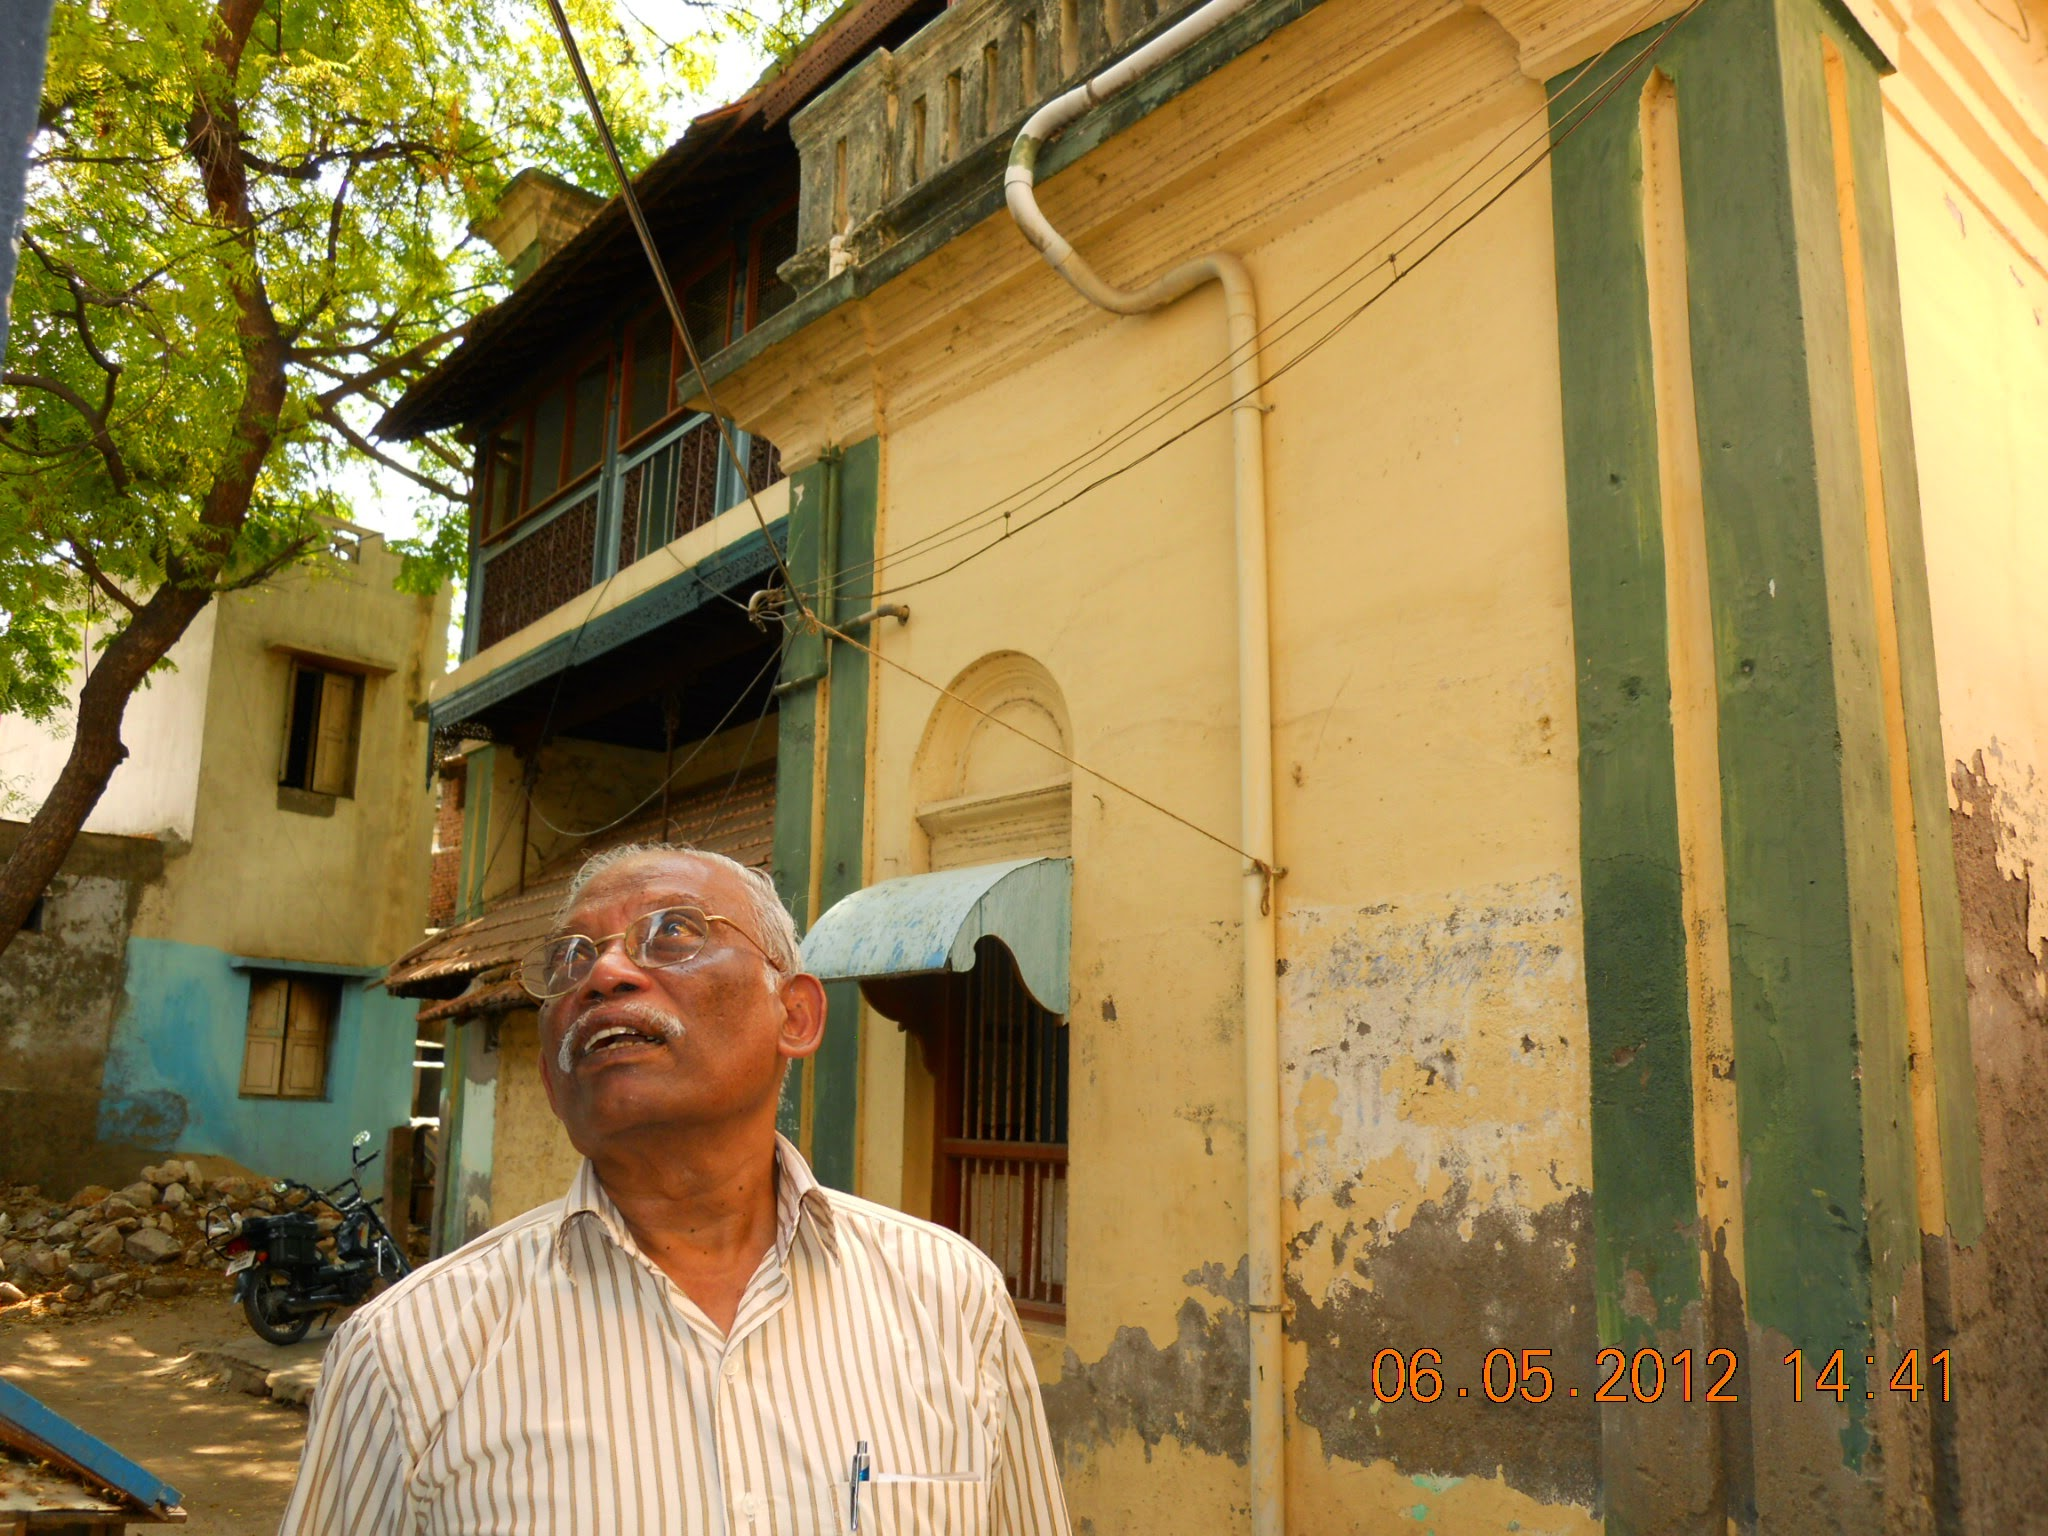
\includegraphics[width=0.7\textwidth]{images/new-images/02-Rajaji-home.jpg}
\caption{Our house at Kamuthi}
\end{figure}
\vspace{-\topsep}

In the beginning we lived in Ramalingam's house. Sometime in the 45-47 
period we moved into a very big house which my\break father took on lease. It 
had two storeys, many rooms and\break terraces. Third storey was a open 
terrace and from there we could see the fort at Kottaimedu, since our 
house was the tallest building in the whole area.

The house had a backyard where we had a cow. We children were afraid of 
going to the backside of the house since it was dark and we did not have 
electricity. Cobras were suspected to be around. A snake charmer was 
called and he caught one cobra from inside one of the rooms at the back 
and one in front of the house where there was an empty space. Some 
people said the snake charmer brought his own cobras and pretended to 
catch them!

One night my father was bitten by a small snake in our\break terrace upstairs, 
but probably it was a non-poisonous snake.

But there were many scorpions and I was stung by them a few times. 
Although it was intense pain, it lasted only twenty four hours! Those 
days, children used to suffer from many\break diseases such as cholera and 
small-pox. Infact, every year in a particular season many children died 
of cholera.


There was one ailment that affected me during every season. 
Every morning when I woke up, the eyes were covered by some discharge 
and it was very painful to wash them. There was a remedy called 
``kaduvudan" which, I think, were the seeds of some plants and these were 
powdered and put into the eyes. It was always done just after midnight 
and operation was always performed by some old ladies (my relatives). It 
was extremely painful, but in the morning, eyes became clear 
miraculously and the ailment was cured.


All these diseases and ailments have disappeared, thanks to advances in 
medical science and better hygiene.
 
Those days the shops remained open even on Sundays. Then the Government 
passed an order that all shops must be closed on Sundays. So every 
Sunday my uncle Ramalingam and a few of his friends (which included 
Periaswamy) used to make poories in the terrace upstairs and it was a 
very enjoyable occasion. Poories were a novelty at that time. In fact 
wheat itself was unknown. During the war rice became scarce and 
government introduced wheat into Tamil Nadu.


Another joyous occasion was full-moon days when my\break mother along with a 
few neighbours used to cook special meals (called koottanchoru) in the 
terrace. All this happened when we were living in my uncle's house.
 
Once I traveled with my brother Rajaguru by bullock cart\break to a 
neighboring village called Kollangulam.\ There Nadar\break community had landed 
property along with a farm-house. My grandfather was working there as 
the man-in-charge. He had invited us there. We spent a whole day and 
night. Recently,\break after more than 70 years I visited Kollangulam with 
Rajaguru.

The Nadar community earned quite a bit of money from\break the land and the 
Muthumariamman Temple was managed with those funds. The community had a 
local government called\break ``uravin murai" which even levied tax called 
``mahamai" from every Nadar family.

The first educated Nadar from Kamuthi was Dr M Natarajan who was the son 
of Mahalingamurthy Nadar who was a formi\-dable character. People have 
seen him beating his son with the stick part of a palm-leaf fan. Once a 
widow was punished by the uravin murai for crossing into the forbidden 
muslim street. He fought against that and the uravin murai decreed he 
should apologize by symbolically breaking a coconut in front of the\break 
deity in the temple. He refused to apologize and the uravin\break murai 
expelled him from the community. He left Kamuthi and thereafter lived in 
Madurai.

After getting MBBS, Natarajan served in the war effort.\break He went to Japan 
and treated the wounded British and Indian mili\-tary men. So he was 
awarded a high military rank. After the war, he settled in Madras and 
became a famous orthopedic surgeon. He rose to become the Principal of 
the Madras Medical College.

Natarajan is a relative of my wife and a distant relative of mine. My 
father used to say that if one wants to get educated he should take 
Natarajan as his model.

Kamuthi was an important market-town for the surroun\-ding villages. Every 
Tuesday Kamuthi became a Sandhai (market). People from the surrounding 
areas came on that day and bought or sold things. This activity took 
place mainly in a special area called Sandhai, located in the southern 
part of Kamuthi. The whole town was full of people on that day. There 
was very brisk business in all the shops including our vessel shop.

\section*{School (1941 to 1952)}

I studied in Kshatriya Nadar Higher Elementary School up to the fourth
standard and in Board High School from fourth to the eleventh standard
which is the end point of school education those days.

\vspace{-\topsep}
\begin{figure}[H]
\centering
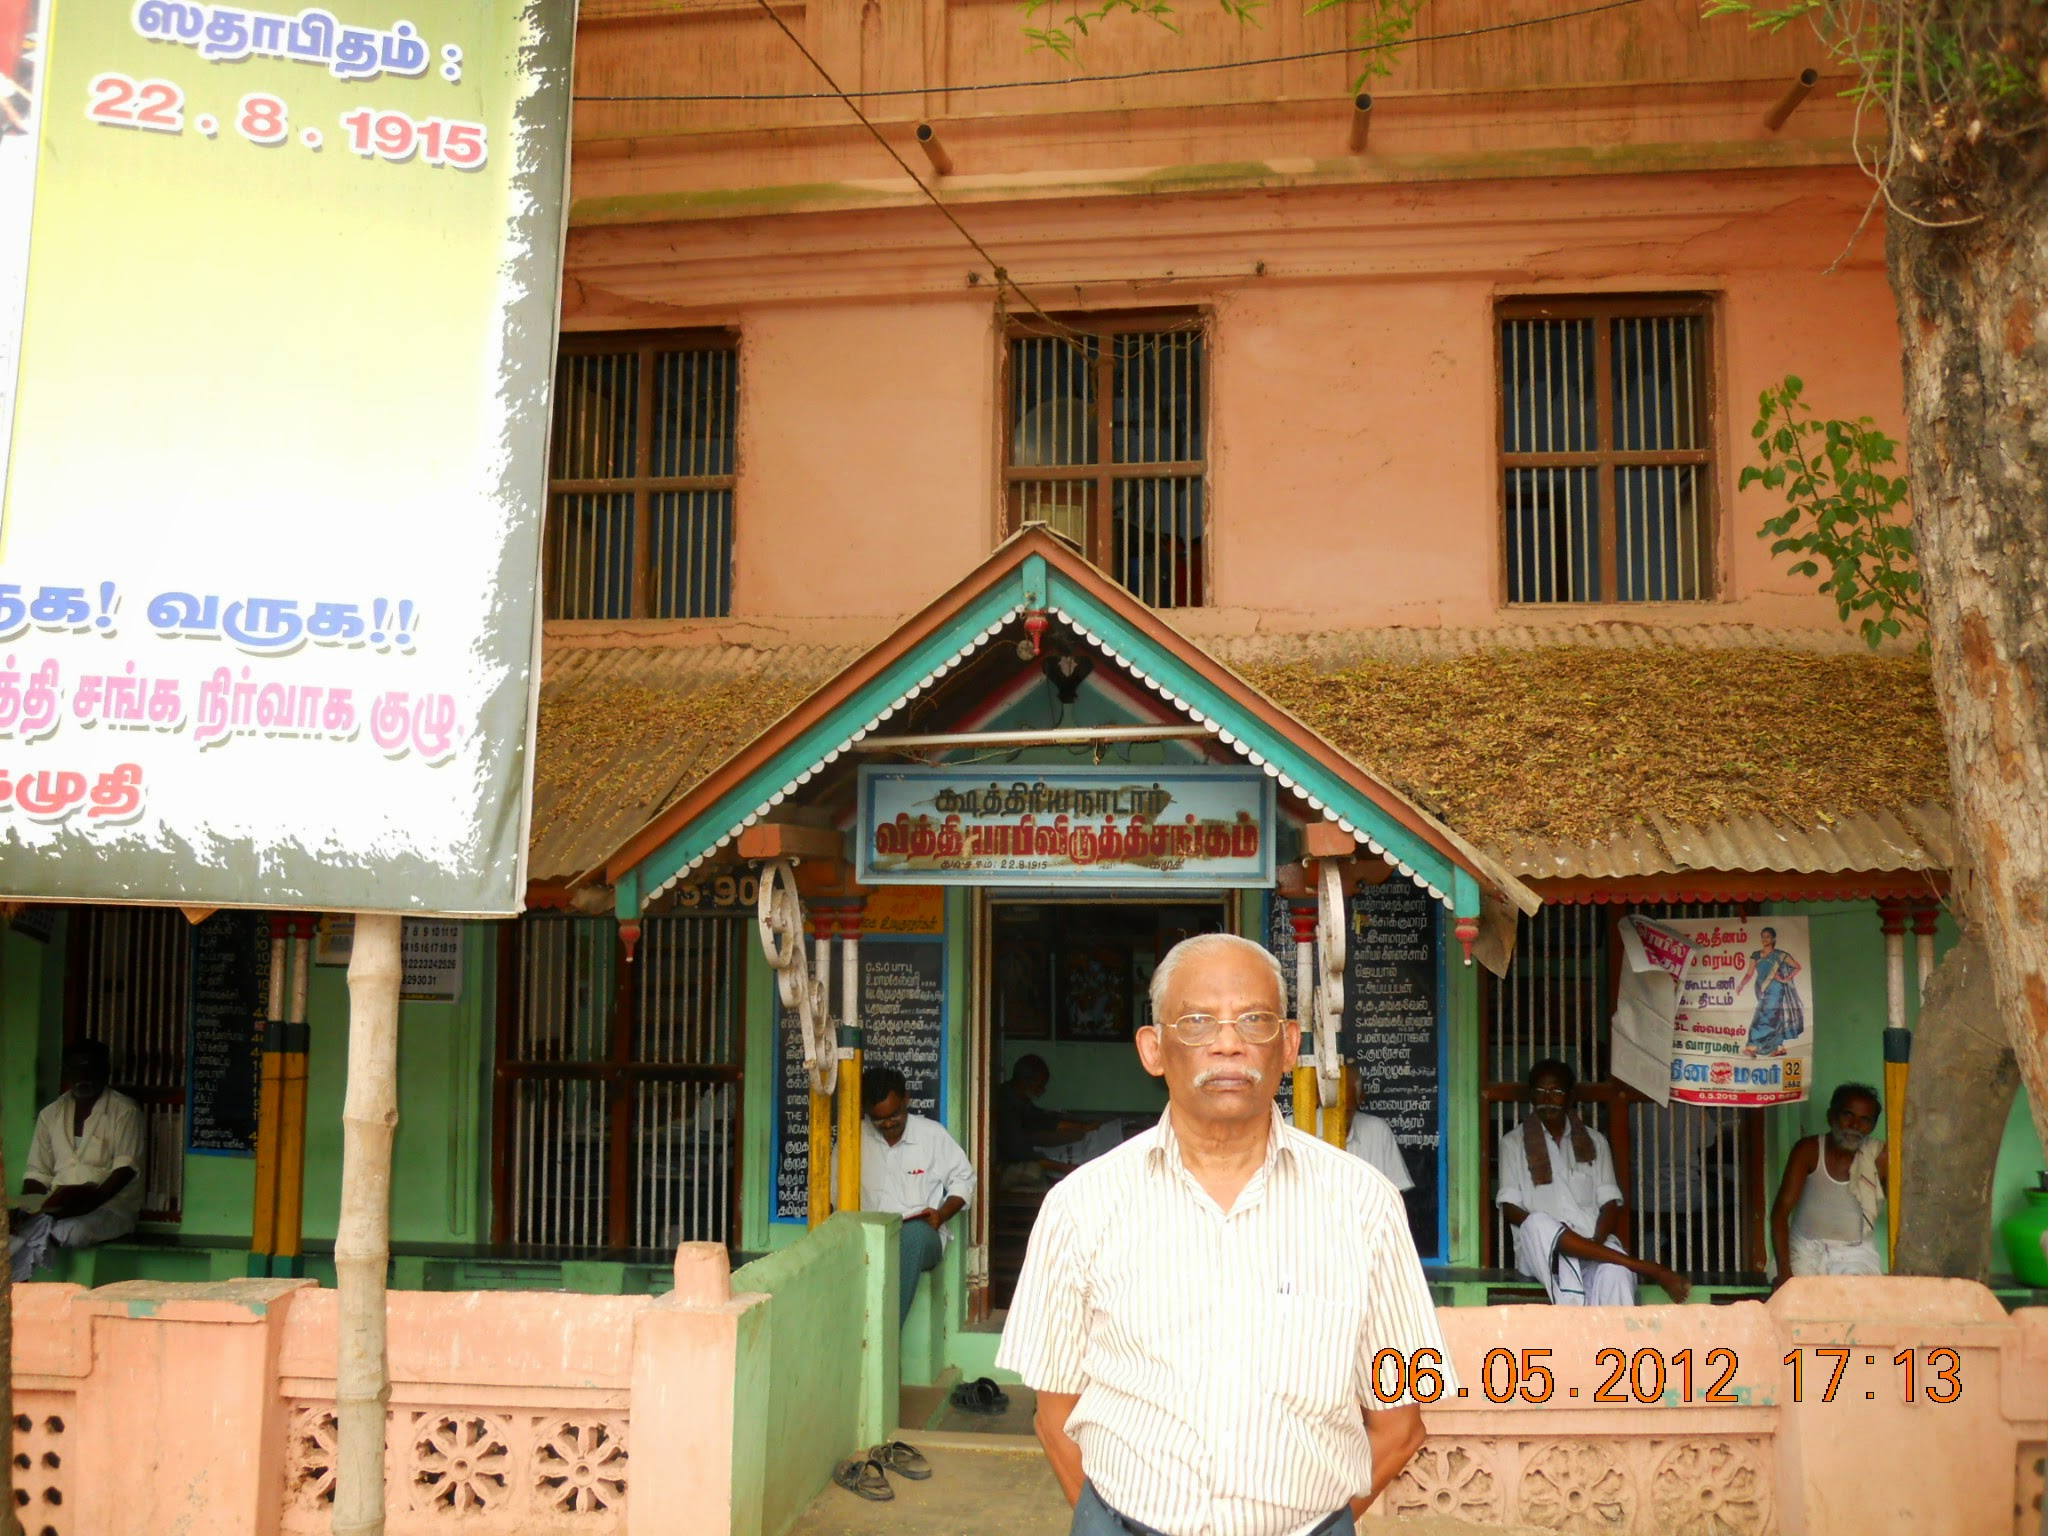
\includegraphics[width=0.8\textwidth]{images/new-images/03-Rajaji-lib.jpg}
\caption{\small{Nadar Vidhyabhiviruthi Sangam (with the\break Library)}}
\end{figure}
\vspace{-\topsep}

Among my teachers in the elementary school, I still remember Ulaganatha
Iyer, Subramania Iyer, Subramania Pillai and\break Alagu Ramaswamy Pillai who
was an excellent teacher.

During the school days, I spent all my time after school, at our shop. 
In fact in my father's absence I have sold many vessels. But my heart was 
not in this business. Since the vessel shop was not busy most of the 
time, I could concentrate on my studies. I came out first usually in 
most subjects.

Apart from the shop, there were two other places which I frequen\-ted. One 
was Muthumariamman Temple and the other was Nadar Vidhyabiviruthy Sangam 
which was a library. There were newspapers and monthly magazines. There 
were old books too. Among them I found a book of science where Thomson's 
atomic model was described. It also contained Michael Faraday's\break 
discovery of electromagnetic induction with excerpts from his\break diary. I 
enjoyed reading them and it created in me an interest in experimental science.

The Sangam was under the care of V Saravana Nadar who was a distant 
relative of mine. He was a bachelor and lived in the Sangam premises.He 
cleaned up the premises and took care of the reading room and the 
library. There was a radio upstairs that was also under his control. 
News by All India Radio and good carnatic music emanated from the horn 
loudspeaker. We got the news about Gandhiji's assassination on 30 
January 1948 from this radio. Our house was a little distant from the 
Sangam, but the direction of the loudspeaker was such that I could hear 
the music sitting on our upstairs window, especially in the nights. 
This was my first encounter with beautiful carnatic music!

Now a guest house with AC rooms and attached bathrooms has been added to 
Sangam and I stay there during my visits to Kamuthi.


I was very much attracted by the Muthumariamman Temple\break which was close 
to my home.\ I liked to watch the priest doing\break pooja to the deity and 
went with the deity in all the temple\break processions during the festivals.
  
In 1945 Germany was defeated in the II World War and it was celebrated 
in India which was under the British rule at that time. So the Union 
Jack was flying over the Tahsildar's office. After a while it was 
removed. I asked my father why was it removed. Like most children I 
liked the colourful flag. My father said in any case it was not our 
flag, we were being ruled by the British. That is the first time I 
became aware that we were not independent.

When I studied there, the Kshatriya Nadar Higher Elementary School had 
only up to eighth standard. It started maybe a century earlier. Later, 
after my time there, this school became a High School with classes up to 
twelve. Although it has the\break Nadar name, it caters to all the castes. 
In fact now most of the students are from the surrounding villages and 
students from other castes, especially Thevars. Hence 
the School administered by the Nadars has been doing good social 
service.

A few years ago, the Nadar School celebrated the Golden\break Jubilee of its 
High School version and I attended it.

\begin{figure}[H]
\centering
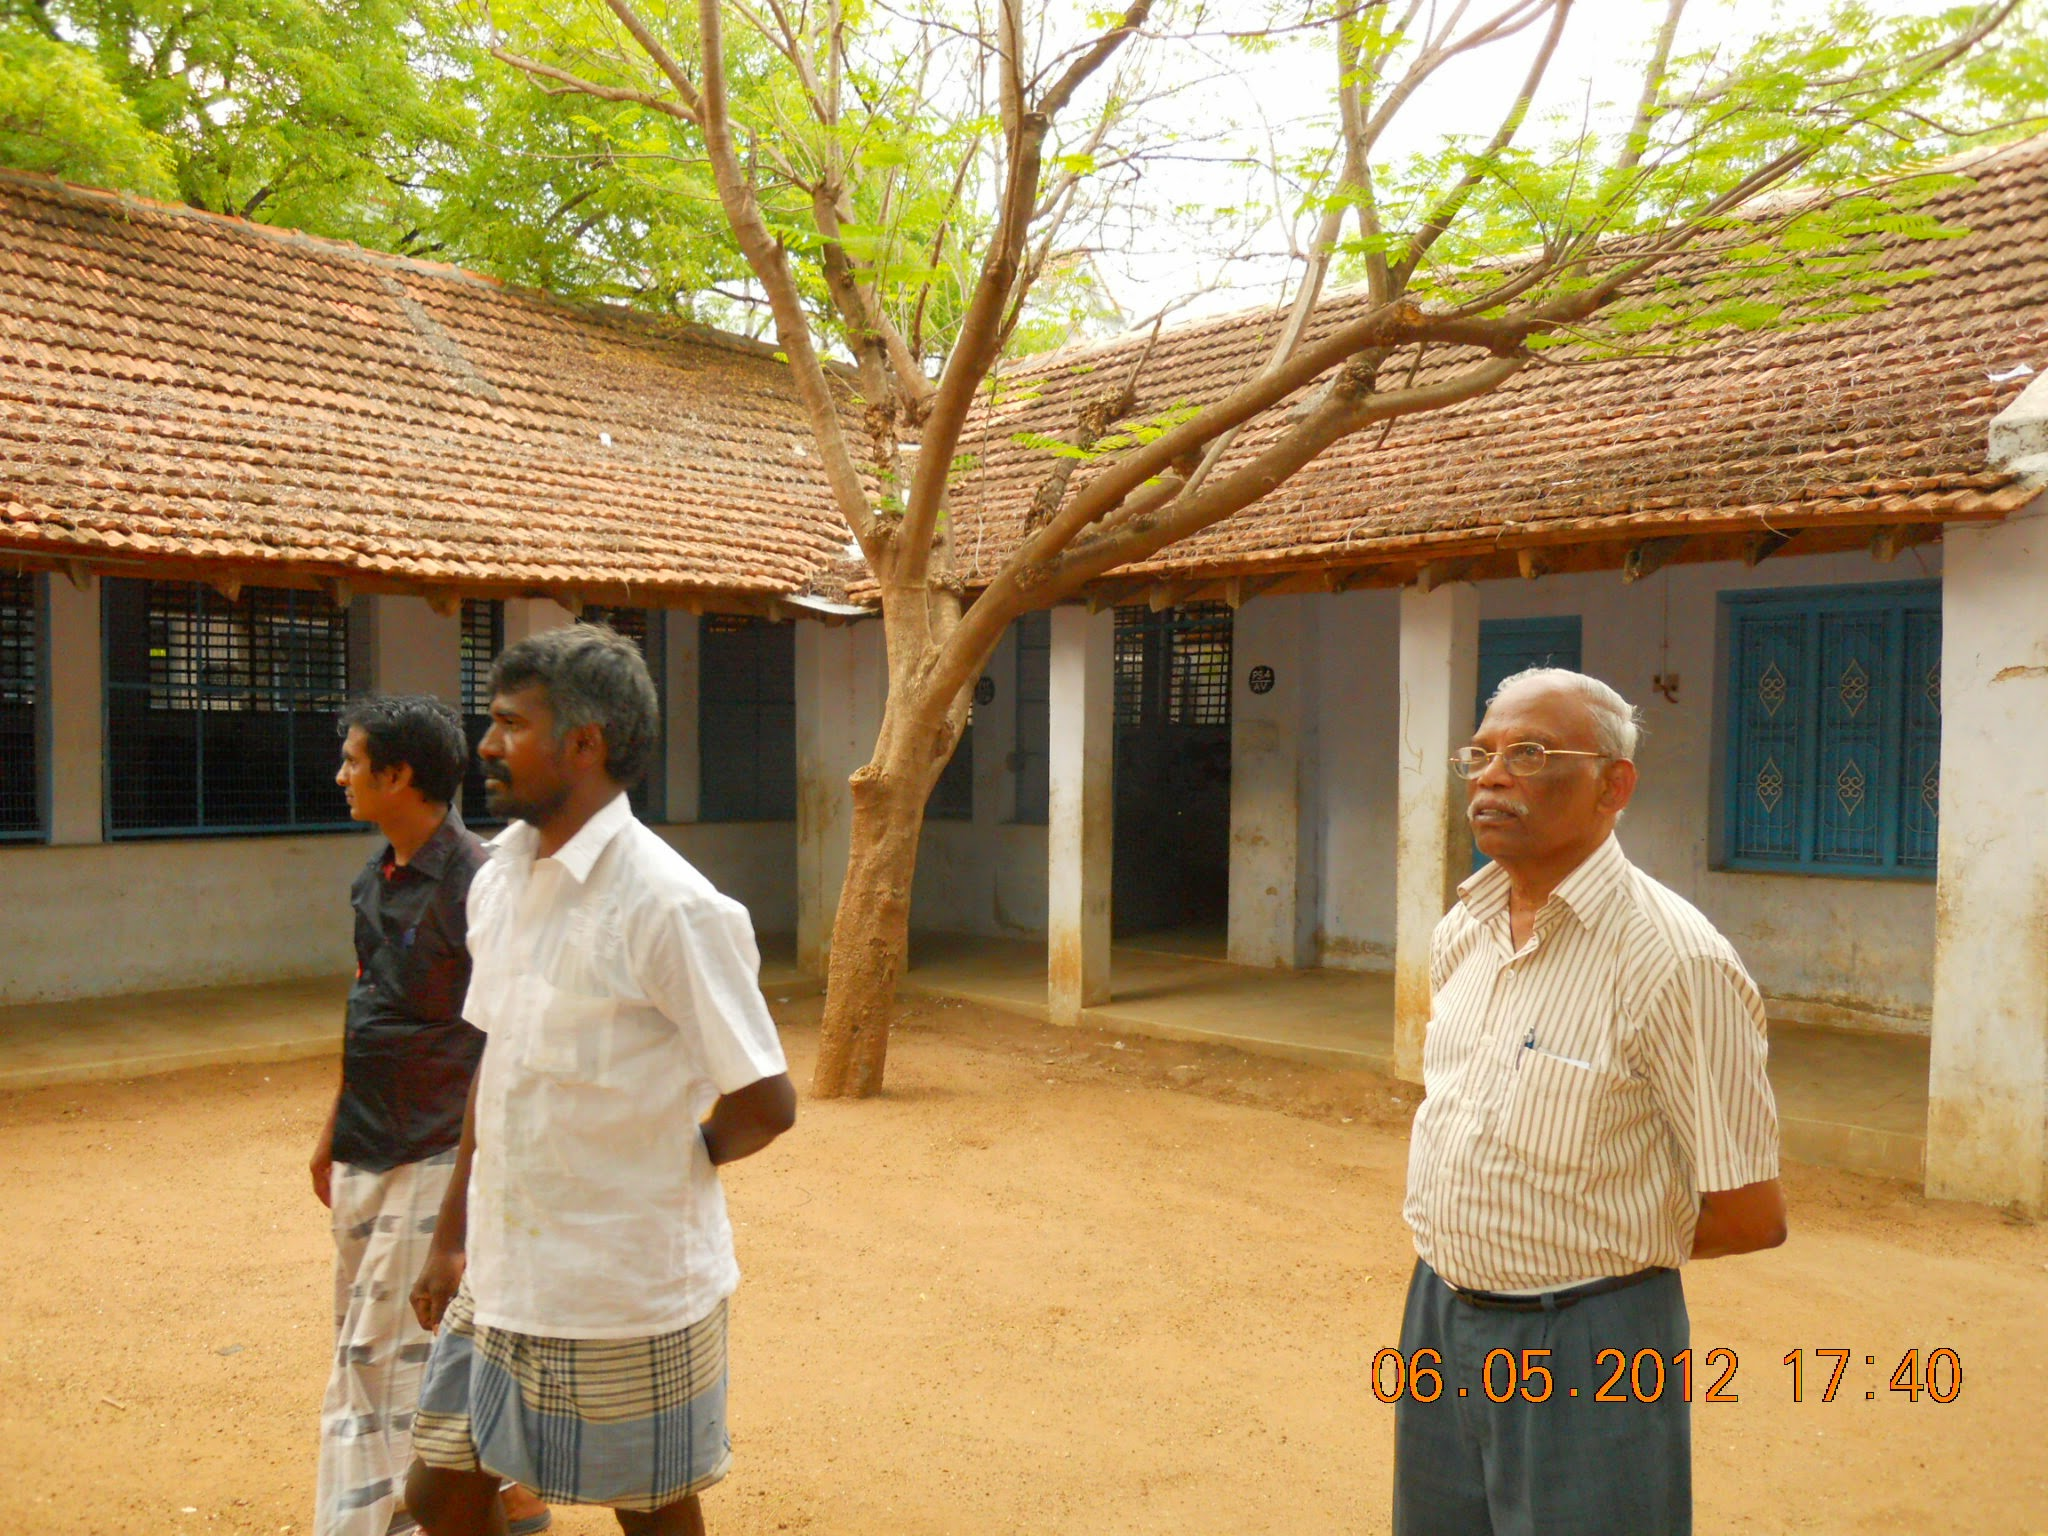
\includegraphics[width=0.8\textwidth]{images/new-images/04-Rajaji-school.jpg}
\caption{\small{Board High School, Kamuthi where I studied.\break I visited it recently.}}
\end{figure}

At school a Muslim boy was saying Gandhi was sent to the jail. I asked 
who was Gandhi. He said he was Jinnah's opponent. That was the first 
time I heard of Gandhi.

Maybe it was 1946.\ There was news that Gandhiji was\break coming to Madurai. 
My father planned to go to Madurai to see Gandhiji. I requested him to 
take me with him and he agreed. But unfortunately, my father could not 
go for some reason and I lost my only opportunity to see Gandhiji.

Actually, it was neither Gandhiji nor Nehru but Netaji\break Subhash Chandra 
Bose who was popular among the youngsters. All of us carried a photo of 
Bose in military uniform in our\break pockets in defiance of the British 
Government who considered that as a punishable offense.

Independence came in 1947 and on that day I was not in\break Kamuthi. My 
father took all of us to Yeral, a pilgrimage town, the same trip which 
was postponed due to the arrival of my grandfather. We were all sleeping 
in the Chathiram of the temple on the night of 14 August 1947. We were 
woken up at midnight\break because they wanted to clean up the Chathiram on 
the eve of the Independence Day. Next morning Lord Subramanya during the 
procession was wearing a garland made of charka-spun threads. That is 
how we celebrated Independence of India.

Since I was a top student in the elementary school, my\break father's friends 
advised him to shift me to the High School after I finished class four. 
When my father took me from the elementary school to put me in the high 
school, it was Chellappandian, the class five teacher in the high school 
who took charge of me. He asked me to write an essay on ``The Cow" in 
English. Since Alagu Ramaswamy Pillai at the Elementary School had 
taught me English, I could write ``The cow has four legs and one 
tail....". Chellappandian admitted me into class five.

Apart from Chellappandian, I had many excellent teachers in the high 
school - Edward Muthuswamy Pillai, Chellam Pillai,\break Karuppaswamy 
Thevar... and above all Subramania Iyer, the\break Head Master and English 
teacher for class eleven (which was called sixth form). The way he 
taught Shakespeare is still\break ringing in my ears! He trained me to act as 
Mark Antony in the Annual Day of the School and my rendering of Antony's 
peroration after Julius Ceaser's assassination was a great success! The 
local doctor Thirunavukkarasu recalled it whenever he saw me and 
congratulated me.

There was a custom of putting up the day's news in\break a black board at the 
morning's prayer meeting at the school. Follo\-wing the Headmaster's 
command, I chose the headlines\break from The HINDU every day and put it up. 
This also gave me good practice in the English language.

There is one incident I cannot forget. In class eight (third form) there 
were two sections taught by Edward and Chellam Pillai. Since Edward had 
impressed me very much as a good and interesting teacher in the second 
form, I wanted to go to the\break section of Edward. But I was put in the 
other section. They did not allow me to change the section since that 
was apparently against the rules. I was very disappointed.

But what happened afterwards proved to be an anticlimax! Chellam Pillai 
turned out to be an excellent teacher. Not only that. Since I was the 
first in the class and especially because he liked me, he made me the 
monitor and put the whole class under me. In the class tests, I was 
asked to invigilate with powers to punish the wrong-doers!

We were taught Tamil by two Tamil Pandits, Koormavatara Konar and then 
Heramba Iyer. Both could compose Tamil poems on the spot. In fact the 
latter when he scolded the students, it was in the form of a poem!

Hindi was taught in the high school, but then the Hindi\break agitation by DMK 
caused the abolition of Hindi teaching. The Hindi Pandit Nagarajan lost 
his job. A few of us who wanted\break to learn Hindi paid Nagarajan and he 
taught us. He was a very good teacher and I passed the Prathamic, 
Madhyama and\break Praveshika examinations conducted by the Dakshina Bharatha 
Hindi Prachar Sabha. I do not remember whether I went for the Rashtra 
Bhasha examination also.

Karuppaswamy Thevar was our manual training (carpentry) teacher. But 
apart from that he taught us Thirukkural since he was a great admirer of 
Thiruvalluvar. He was also a staunch advoca\-te of vegetarianism, but more 
on that later.
 
A big problem with the high school was the absence of good teachers for 
science. Since Kamuthi was a backward area, even the teachers who joined 
left soon. We did not have a teacher for Maths. As a result my school 
abandoned Algebra and Geometry and only Arithmetic was taught. Algebra 
and Geometry were called Composite Mathematics and it was not done. So 
when I go to College I would not be eligible for First Group 
(Mathematics, Physics and Chemistry). But my good Headmaster advised my 
father to buy the standard text books on Algebra and Geometry and 
advised me to learn them by myself. This is how I spent my vacations.

So my knowledge of Mathematics had many gaps. In spite of that I got 
first group in the College.

The High School was situated at the southern end of the\break town. It was 
just thatched sheds. When I had completed the High School, it shifted to 
pukka buildings to the north of\break the town, at Kottaimedu. The Chief 
Minister inaugurated it. It continued for many years, but now I hear it 
has been converted into a College!

When I was in Kamuthi recently, I had a surprise. I went with my brother 
Krishnamoorthy to the location where my old school in thatched shed was 
situated. It was still there! Actually after the Board High School 
shifted to Kottaimedu, the shed housed a Muslim School. That also 
shifted and they were going to demo\-lish the shed, but they had not done 
it when I visited. So I was very lucky to see my old school!

We had a cow at home. The cow and its calf were sent\break outside the town 
for grazing every day. One day the cow alone returned. It was noticed 
fairly late in the night. My father and myself went with a torch and we 
could locate the poor calf which was huddling against a wall. Every one 
was happy to see the calf.
\vskip 1pt
Another time, I lost my gold ring while playing football in the high 
school. Again it was noticed only late in the night. My father and 
myself went to the football ground in the high school. Even though the 
football field was very big, I managed to find the ring!
\vskip 1pt
There was no electrical connection at our home, but the\break shop had it. So 
not only myself, but all my brothers and\break sisters also studied in the 
evenings at my shop. But my studies\- continued even after the shop was 
closed, especially during the exam period. So I used to study in the 
light of a kerosene lamp sitting in the bed. Once I fell asleep and the 
open kerosene lamp fell. A serious accident was averted only because my 
parents\break noticed it in time. After that I was forbidden to study in the 
bed.

I passed out the government examination, called SSLC\break (Secondary School 
Leaving Certificate) exam, with good marks and went to study 
Intermediate in The American College in 1952. This was a big step in our 
family. By that time our shop was not doing well and my father needed me 
to help him. My uncle who was helping him in the shop left him and 
started his own vessels shop which was a rival to our shop. My mother 
did not like my going away. But my father wanted me to pursue higher 
education. His idea of higher education was either to go for the IAS 
examination or start a big business with the help of my education.

Where can the money for my higher education come\break from? Clearly my father 
could not afford it. I got a loan scholar\-ship from Nadar Mahajana Sangam 
which had to be repaid. I also got a merit-cum-means aid from the Madras 
Government. None of this was enough since the hostel expenses were high. 
My\break father had to take it from our shop which went down further as a 
consequence. Later I could compensate him but that was much later. Even 
from my Training School stipend of Rs.150, I could send him a large part 
of it. I continued to do it from my TIFR salary. Since TIFR continued to 
pay my research assistant salary when they sent me to Chicago I sent him 
the whole of it. Not only that. I saved a large part of my assistantship 
money in Chicago and sent it. As a consequence he could build a new 
house. Until then we did not own a house.

One reason our shop did not do well was this: my father bought some land 
and he could not concentrate on the shop. From land also he did not get 
any income since we were in a rain-deficient region.

Among my brothers only one, G Krishnamoorthy could\break rise high in 
education. He became a Professor in TIFR. He\break was financially supported 
by me after I began to earn. Another, Arunachalam also was supported by 
me and he got employed in a bank. The oldest of my brothers, Rajaguru 
became a successful\break businessman. He along with his three sons became 
manufactu\-rers and traders of furniture at Madras. Ramachandran did not 
study well and never did anything. He died some time ago.\break Among my 
sisters none completed school education although two of them did very 
well in elementary school. Unfortunately, my mother stood against their 
education and even my father could not do anything.

Actually after my father's time I wanted that our house and other landed 
property must go to my sisters only since none of them was well-to-do.  
My mother and brothers did not agree and did not want any part of it to 
go to my sisters. I did not want to take any part of it although the 
house was built solely from my money. I cut off all connection with all 
of them and Kamuthi.\break After many years, all this has been forgotten and 
now I have good relationship with all of them. I went back to Kamuthi 
only after 40 years!

\vspace{-\topsep}
\section*{The American College, Madurai (1952 to 1954)}
\vspace{-\topsep}
Intermediate was roughly equivalent to the present plus two. In spite of 
some gaps in my Mathematics, I was admitted to the first group 
consisting of Maths, Physics and Chemistry.

\vspace{-\topsep}
\begin{figure}[H]
\centering
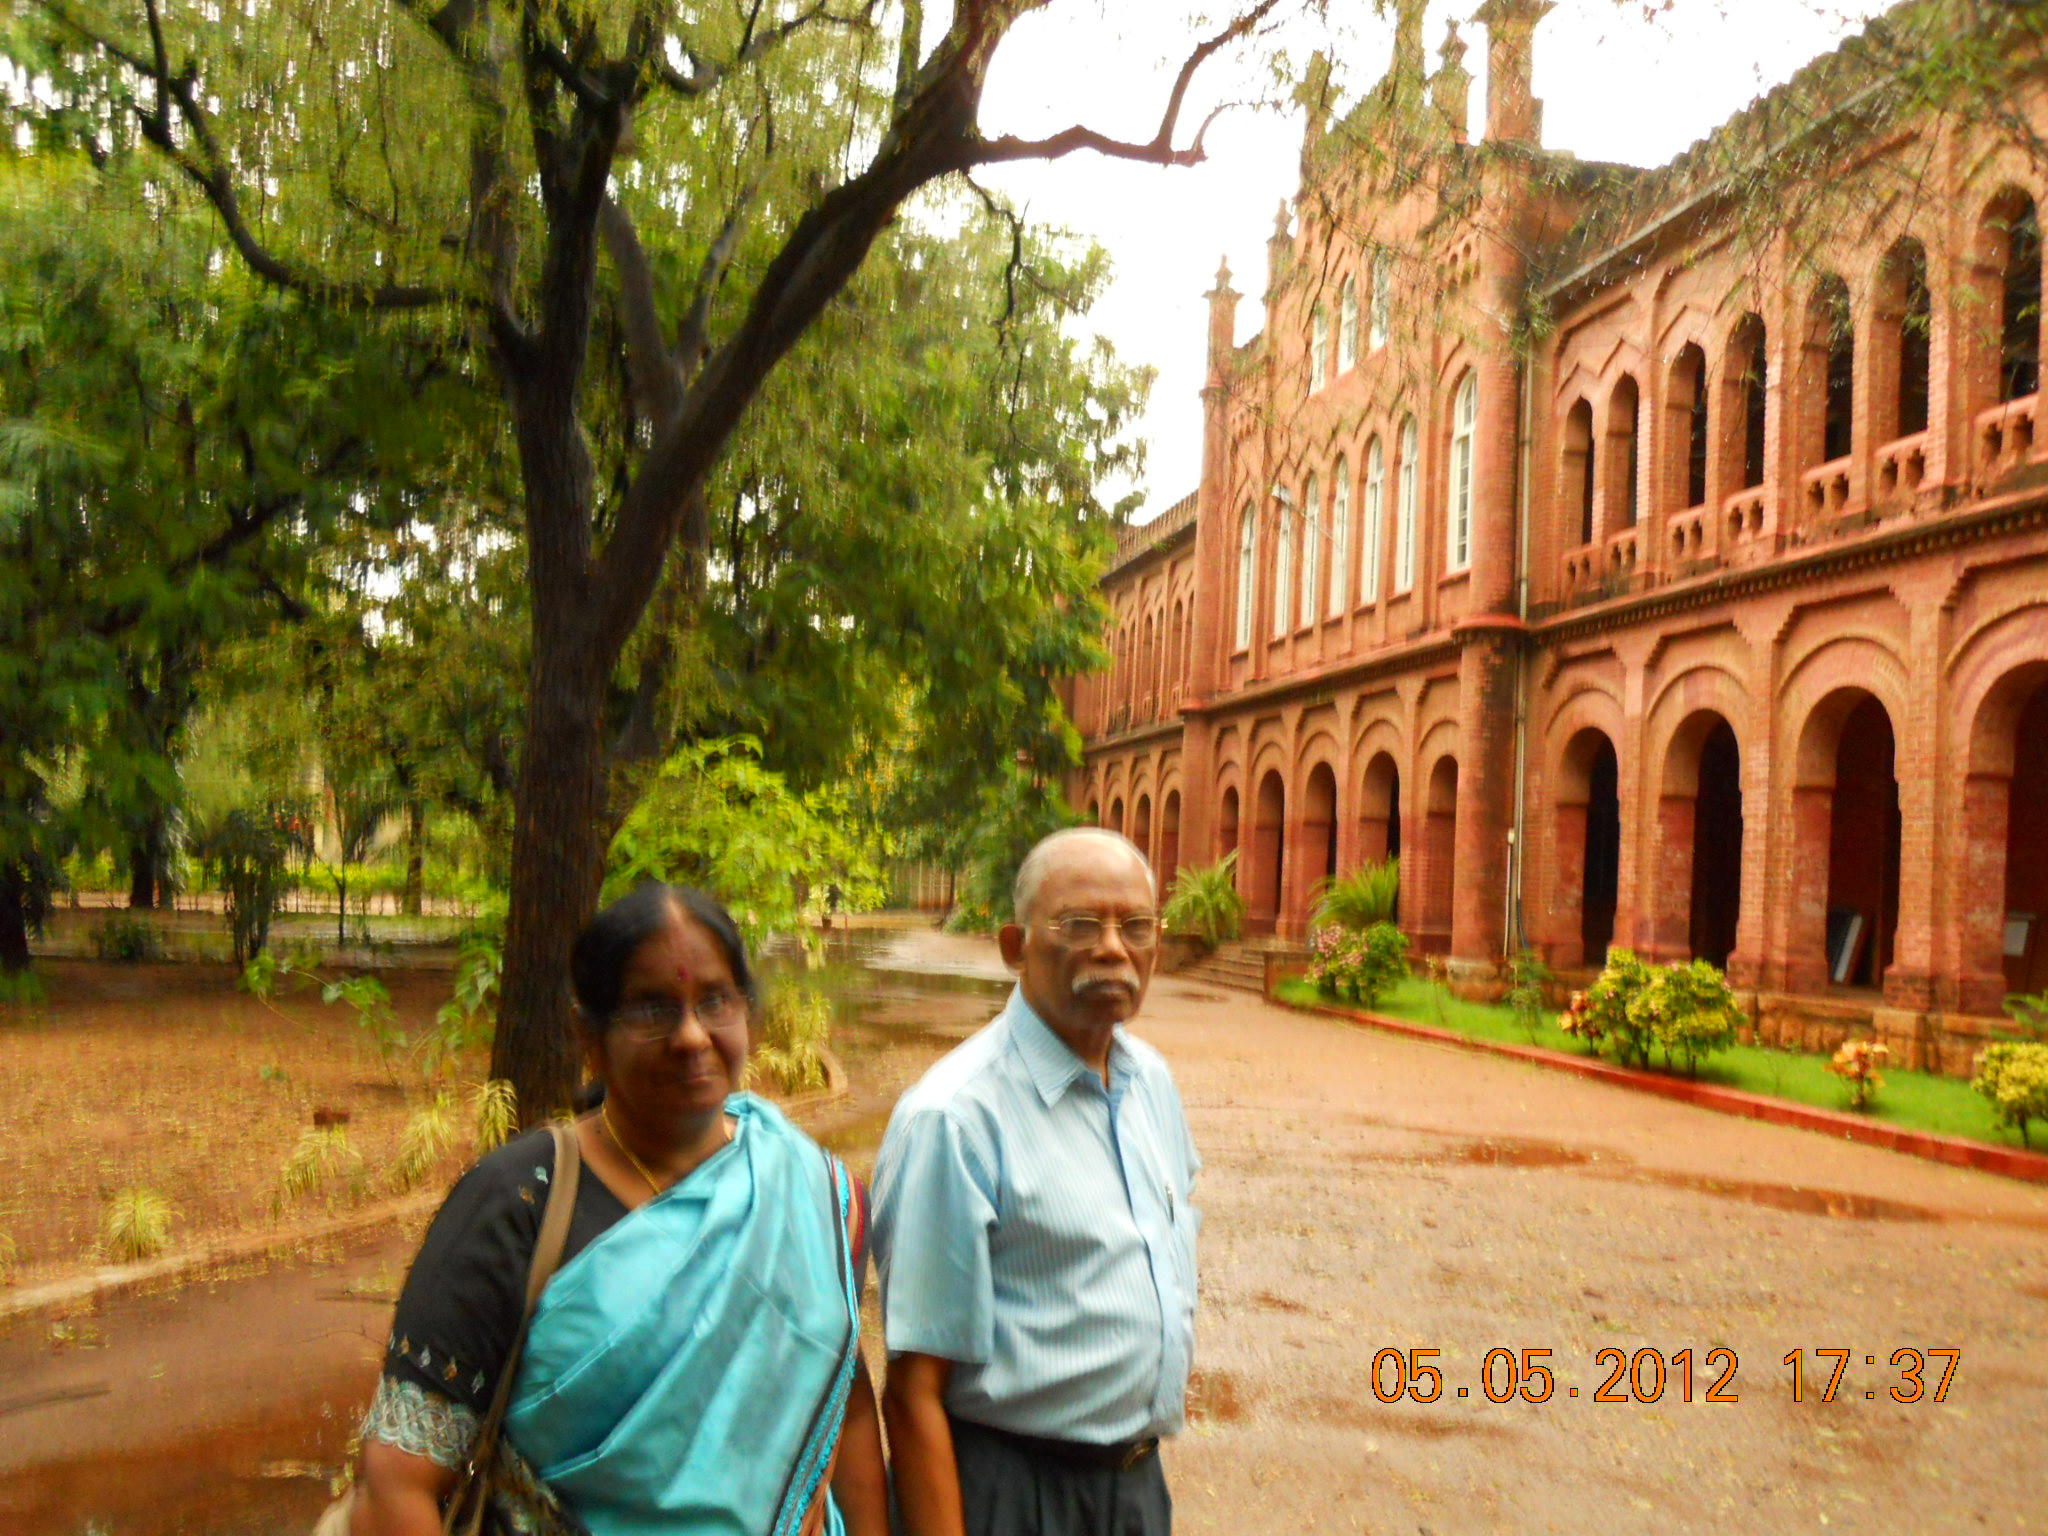
\includegraphics[width=0.6\textwidth]{images/new-images/05-Rajaji-AC.jpg}
\caption{\small{American College, Office building}}
\end{figure}
\vspace{-\topsep}
\newpage

American College was an exhilarating experience for me.\break The stately 
buildings and the excellent faculty of the college\break impressed me very 
much. I stayed in the Wallace Hall which was one of the three hostels. 
ES Moses taught me physics and\break Ramaswamy taught me chemistry. I have 
preserved the exce\-llent notes of Ramaswa\-my's lectures that I took. T 
Natarajan, Benjamin Guna\-raj, Gift Siromoney and a few other very good 
teachers taught mathematics.

I had two very good friends in the college. K S Ramakrishnan who went 
for IAS and later resigned because of his honesty. I have very good 
contact with him. The other, M Pathamuthu became a Gandhian and lives in 
a village near Madurai.

It may be 1953 or 54, Nehru visited Madurai. I had come home on 
vacation. I wanted to see Nehru. My father permitted\- me to go. The whole 
temple city was decorated to welcome\break Nehru. He was supposed to pass 
through the road in front of American College. My friend Pathamuthu and 
myself stationed ourselves at a vantage point inside the college campus. 
When Nehru's car came near the college, a group of DMK fellows threw 
something at Nehru's face. It was stones inside a black cloth. For a 
moment Nehru's face showed his pain but his smiling face appea\-red soon. 
I hated this barbaric act by some of the MCC studen\-ts.

During one weekend, myself and a few friends (Pathamuthu, Sakthivel and 
Solaivasaham) went on a trip to the Alagar Koil which was in a 
neighboring hill to the north of Madurai. It was a nice picnic.

Alagar Koil is a famous temple for Lord Vishnu (Alagar).\break During the 
Chithirai festival of the Meenakshi Temple, Alagar comes down to 
Madurai and in the early morning enters into the river Vaigai. Lakhs of 
people come to witness this event.

During a recent visit to Madurai, I was lucky to witness this event of 
Alagar entering Vaigai.

It is said that Alagar, that is Vishnu, being the elder brother of 
Meenakshi, was coming down to give her away in marriage to Lord Shiva. 
But Vaigai was in floods and he was delayed. The marriage was held 
without him and Alagar returned to his abode in anger.
 
There was religious instruction for Christians and moral\break instruction for 
others. My moral instruction class was taken by an Economics Professor 
KJ Charles. His lectures were fantastic.\break He lectured on Marcus Aurelius, 
Thomas Aquinas and Albert\break Einstein. I learnt about Einstein in a moral 
instruction class!

But I had heard Einsteins's name from my Tamil Text book in the high 
school. Mu Varadarasanar's article mentioned the famous lines of Kaniyan 
Poongunranar in a Purananuru poem ``Yathum ooray, yavarum kelir"
(All places are mine and all are my relatives).
and called the poet the Einstein of social sciences!   


A crucial event occurred during the American College\break period. A friend 
took me to watch the night sky from the terrace\- of the Mathematics 
building. It is a look through the College telescope that determined my 
trajectory in this life.


It just happened that it was the best time to observe\break the Moon. When it 
is dark of course you cannot view it and\break when it is fully bright it does 
not show its features clearly. But that day was the half-way point 
between New Moon and Full Moon days. The shadows cast by the mountains 
in the Moon got\ elongated, with sharp edges. I felt as if I was standing 
on\break an elevated height above the Moon, looking down. It was so 
frightening, the mountains and craters.\ It was a fantastic\break experience. I 
realized.


``There were more things in Heaven and Earth than were dreamt of in my 
philosophy".


Since Science alone held the key to these other ``things" I had no 
hesitation in my choice of what I wanted to do. I am\break sure many others 
too have \,been \,lured \,into \,Science \,through Astronomy.


I went to the Daniel Poor Library (It was not a poor\break library at all! 
Poor was the name of the donor of the library in the College. It was a 
well-provided library.) and borrowed many interesting books. Eddington's 
(or is it James Jeans) ``Expanding Universe", George Gamow's ``Life and 
death of the Sun" are some of the books that I read and enjoyed. My 
interest in Astronomy and Physics increased further. I published my 
first article ``The Mysterious Universe" in the College magazine.

At the end of my intermediate in 1954, it was clear to me what I should 
do. I must pursue Physics. In those days Madras University had a 
programme for keen students called Honours. But it was offered in very 
few colleges and it was tough to get in. My father of course agreed, 
in spite of my mother's objections.
\vspace{-\topsep}
\section*{Madras Christian College (1954 to 1957)}

B Sc (Hons) in Physics was offered in St Joseph's College,\break Trichy, 
Madras Christian College and Presidency College. I\break applied to St, 
Joseph's and Christian. I got admission in St\break Joseph's. I had secured 
very good marks in the intermediate exam, so I should have got admission 
in Christian College\break also which is the preferred choice.  There were 
postal delays in getting my marks from Madras to Kamuthi and then from\break 
Kamuthi to the College. The eleven seats in Christian were\break already 
filled. So I was offered Maths Hons. But I was told that I can shift to 
Physics if a vacancy arises due to someone leaving for engineering.

I decided to take the chance at Madras Christian College\break  (MCC). I 
attended the Maths Hons class but the lectures were too dull for me. 
Everyday I went to the Principal's office and\break enquired about the Physics 
seat. The Principal's secretary Ernest will tell me as soon as he saw my 
head at the window ``No". I was getting frustrated. Meanwhile there was 
pressure from my mother to return and look after the shop.

After many weeks, the miracle happened. The secretary told me that Mr 
Kannan has left BSc (Hons) to join Engineering\break College. I felt Lord 
Krishna (Kannan, in Tamil) Himself came and rescued me!

I got what I wanted and concentrated on Physics. The\break lectures by PK 
John, SS Thanaraj, CB Rajagopal, KB Rajangam and above all, Dr MA 
Thangaraj were excellent. KB Rajangam taught Bohr's model of the Atom 
and it was so good. I cannot forget them. After that, Thangaraj the Head 
of the Department taught Quantum Mechanics. He used Rojansky's book. 
Those days (1956-57) that was the only book on Quantum Mechanics.

The books that I liked were Modern Physics by Richtmayer and Kennard, 
Heat and Thermodynamics by Saha and Srivastava and Properties of Matter 
by Newman and Searle. The last book had many problems and I enjoyed 
solving them during vacation. They were not mere numerical problems. The 
problem had to be formulated in terms of equations which had to be 
solved.

Thangaraj also taught Wireless and Electronics. That was\break the only 
subject that I did not like, although that was supposed be the special 
subject in our Hons course. Every other subject was taught as Physics, 
but this was taught more like an\break engineering subject, just a set of 
prescriptions. Instead of using the standard prescribed text book by 
Terman, he was teaching from the Admiralty Handbook of the British Navy! 
In the Wireless and Electronics exam, I almost failed. Thangaraj was 
also my hostel warden. He called for me in the hostel next morning and 
scolded me thoroughly. For a big question I had answered but had crossed 
it out. He said it was a correct answer and I should not have cancelled 
it. But he passed me nevertheless!
\vskip 1pt
During 1956-57 the syllabus changed and MA Thangaraj\break found that none of 
the faculty could teach according to the\break new syllabus which was 
considerably advanced. He assigned\break the tutor TN Seshan to teach all the 
subjects to us in the final year of the course. Seshan did a marvelous 
job. Later he passed the IAS exam with first rank and became a very 
famous (but not popular) administrator. The high point of his career was 
as Chief Election\- Commissioner when he reformed the whole election 
process in India.


On weak ends I traveled from Tambaram to Thiruvallikkeni and went to 
the University Library. Among the things that I read there were the 
original papers of Rutherford discovering the atomic nucleus through 
scattering by alpha particles and Niels Bohr proposing his model of the 
atom. It was a special fascina\-tion to read these classic papers.
 
The specialty of the MCC (Madras Christian College) situated in 
Tambaram, a suburb of Madras was the Hostel system. There were three 
hostels St Thomas Hall, Bishop Heber Hall and\break Selaiyur Hall. I belonged 
to St Thomas. Not only the out-of-station students but the so-called 
day-scholars also belonged to one of these halls and developed an 
affinity towards the hall to which the student belonged. Only the 
lectures and laboratories were in the College. All the extra-curricular 
activities were in the halls. I had two classmates who were my friends 
Ratna\-prabhu and Mahalingam. Ratnaprabhu became a textile engineer and 
rose to the level of the Director of Ahmadabad Textile Institute and 
Mahalingam became an officer of Indian Airports Authority.

On a Hostel Day, MK Thiagaraja Bhagavathar was invited. He talked and 
sang. I regret that I did not talk to him. For, later I became a fervent 
admirer of his devotional songs. His golden voice captivates me. There 
is none like him.


While at MCC we had to attend intercollegiate lectures\break at Presidency 
College and Alagappa College of Technology. Two series of lectures were 
memorable.\ One was by G N Rama\break{chandran} who lectured on General Theory of 
Relativity(GTR)\break although I was still not academically mature enough to 
understand GTR fully. The other was by Alladi Ramakrishnan who\break lectured 
on the Matrix version of Quantum Mechanics which had not been taught at 
MCC. He was such a powerful lecturer that I was impressed very much.

Here also there were moral instruction classes; they were taken by 
Kibble, a Professor of Mathematics. He used to let us do anything 
quietly when he was looking at his book! There is a good story about his 
absent- mindedness. One day he wanted to go to the city and boarded the 
electric train. He took his book and began to read. After a few hours he 
noticed that he was still in Tambaram station. He accosted a railway 
official and asked him why the train did not leave after so many hours. 
The official said ``Professor, the train has made two trips to Beach 
station!". That was Professor Kibble.

 
His son is the famous theoretical physicist TWB Kibble	who was born in 
Tambaram and spent his childhood in the MCC\break campus. He is the author of 
the nonabelian version of the\break famous Higgs mechanism.\ Later during the 
Golden Jubilee\break celebration of IMSc, I invited him to the Institute and 
took him to MCC where he enjoyed seeing the places of his childhood 
days. He could even identify the tree which he used to climb!

  
I was staying at St Thomas with Villimadan, also from\break Kamuthi, one year 
senior to me.\ One day Karuppaswamy\break Thevar, our teacher from Kamuthi 
visited us. We hid the fact that we ate at the non-vegetarian mess and 
took him to the veg mess. The fact that I had to hide the truth from my 
teacher affect\-ed me very much.


Apart from the above, there were other things. At home every\-body was a 
non-veg. Since I was the eldest son, I was sent to buy meat. I had to go 
every Wednesday to the slaughter-house. One day I witnessed a goat being 
slaughtered. I saw my mother putting live fish (ayirai meen) into 
boiling water. Every Deepa\-vali day in the early morning my mother would 
cut the neck of our pet hen which was screeching. All these events, 
along with the teachings of Buddha, Gandhi and Thiruvalluvar made me to 
take the following step.

\vskip 1pt
I shifted to the veg mess. But when I went home on vacation, my father 
learnt about it and chided me and compelled me to shift back to non-veg 
mess. I had to do it. He said vegetarianism will ruin my health. I 
argued by citing the example of brahmins and others who were 
vegetarians. He would not agree.


So I had to take non-veg food and could become a vegetarian only after I 
went to Bombay and so became free of my father's influence.

 
A tragic event took place in 1956. My friend Villimadan\break died in the big 
train crash. The Thoothukkudi Express fell\break down from the bridge at 
Ariyaloor with considerable number of deaths. Villimadan perished in 
that. He was on his way to a job interview. After hearing of this 
accident, the Minister for Railways Lal Bahadur Sastri immediately 
resigned. Such honesty and selflessness has been very rare in Indian 
political circles.


In the year 1956, it was announced that CV Raman was going to lecture at 
the Presidency College. Thangaraj asked us to go and attend the lecture. 
I think he also attended.


Raman lectured on his theory of specific heat based on the discrete 
frequencies of the crystal vibrations and contrasted it with the 
continuum theory of Peter Debye. At one point his voice rose and he said 
``Debye's theory is not worth the paper on which it is written". So 
saying, he threw the sheaves of paper in his hand and they flew over our 
head and fell into the waste basket. We were all very much impressed. 
Bored as we were with many uninspiring lectures in the class rooms, we 
felt this is how lectures must be given!

\vskip 1pt
The examinations were very tough.\ I had to revise the\break whole subject and 
keep it in my fingertips, otherwise there was hardly any time to 
complete the paper. So, many times I used to stay awake whole night 
before the exam. Such a thing happened before the Electricity and 
Magnetism paper which was the last one. After the exams I went to 
Kamuthi and there one morning I noticed that my eye-balls did not move. 
For seeing anything which was a little to the right or left, I had to 
move my head! My parents became alarmed and it was decided that next day 
I must be taken to the famous Dr Joseph's eye-hospital at Trichy. Those 
days that was the only place for eye ailments. But miraculously, the 
next day my eyes became completely normal!

While I was in MCC, scientists from TIFR (Tata Institute of Fundamental 
Research, Bombay) conducted many cosmic ray experiments in the College 
grounds. They sent up balloons to the upper atmosphere and recovered the 
instrument package\break after many hours. The instrument was special 
photographic\break emulsion that recorded the cosmic ray particle tracks. So I\break 
had the opportunity to meet many TIFR scientists who visited the College 
and gave lectures. Bernard Peters, MGK Menon, RR Daniel, D Lal, Gokhale, 
G Venkataraman. PJ Lavakare. I decided to pursue research in TIFR.

Thangaraj had a research project on Cosmic Rays. He sent nuclear 
emulsion up by baloon and recovered them after a while. The emulsion 
contained the tracks of particles that he studied with some research 
assistants. To recover the baloon one has to track it during its flight 
and note the direction of its fall. Once a baloon was almost lost and he 
asked his students to search for it. We were lying on our back on the 
terrace of the meteorological observatory of the Meenambakkam airport 
and peering through binoculars. I succeeded in sighting the baloon and 
so later it could be recovered! Everybody including Thangaraj was happy.
\vspace{-\topsep}
\section*{The Training School (1957 to 1958)}

Homi Bhabha had this great idea of the Training School where he could develop the human resources needed for the Atomic Energy Programme instead of taking away scientists from the existing scientific establishments and universities.   

It is now called BARC Training School, but the name at\break that time was AEETTS (Atomic Energy Establishment, Trombay, Training School) and it was to start in August 1957. So it was just right for me since I had completed my Hons degree at that time.

I applied and was called for interview in Bombay. I did the interview 
well, but admission letter did not come. Got frustrated and went to 
American College for interview for the physics\break lecturer's job. S J 
Savarirayan was the Principal and Head of the Physics Department. After 
the interview, he asked me to join immedi\-ately. I told him that I am 
expecting a call from Department of Atomic Energy Training School. If I 
do not get it, I will come. He was greatly surprised: I am offering you 
a lecturer's post straight after your degree and you want to go to some 
school! He had not heard of Department of Atomic Energy those days! 

Finally I got the letter from Bombay and joined the\break Training School. Bhabha chose Dr Raja Ramanna to be in-charge of the Training School, and chose Dr K K Damodaran to be its\break active head. Dr Damodaran organised all the daily activities of the School and took good care of all of us. We (the trainees) used to refer to him as the ``Headmaster" of the School (among ourselves), but he was much more than that, he was almost the local guardian for all of us.
 
Bhabha had a predilection for appointing military men as admini\-strators. Perhaps he felt that only military men could\break control the unruly crowd that we were! He appointed a military person Suraj Prakash as our warden. I remember him as a tall and handsome young man, but there was some problem and he was rather unceremoniously replaced by Colonel Ottley. More about the Colonel later.

Bhabha gave an inspiring lecture on the opening day of the Training School. He talked about his dream of bringing nuclear energy to this country and told us how he expected the trainees to help to realize that dream. But at the end of his talk which was aimed at the sky, we were brought down to earth by a question from the audience (namely  one of my would-be trainee collea\-gues). He asked what job we were going to get, after the training period. Nowadays it is common to find that young people are mostly career-minded. They want to know what they will get after one year and what after 5 years etc. Asking for the so called career-profile has become the standard procedure. Fifty years ago that was not the done thing. Most of us had our mind on the sky and were not practical-minded. That was why we were taken aback by the above question from our colleague. But  Bhabha answered the question very effectively. He said the questioner can take his (Bhabha's) job if he proves himself! Bhabha was not bluffing, for a trainee from the 6th batch of the School (Dr Anil Kakodkar) became the DAE Chief, although Bhabha himself did not live to see that.


Our hostel was at Land's End, Bandra. It was really Land's End! The road ended and the sea started. In between the\break end of the road (where there was a band stand) and the sea coast full of black rocks characteristic of the Bombay coastline, there stood rows of military barracks which had been in use during the second world war. Each building had a spartan simplicity:\break four walls mounted by a semi-cylindrical ceiling made of\break corrugated iron sheet. This was partitioned into two rooms and each room contained two trainees. This was the Training School\break hostel to be compared to the present sleek multi-storey building in Anushakthi Nagar.

The classes were held in the Churchgate area, either in\break the Jai Hind College or in the K C College. Some classes were\break also held in the new TIFR building that was coming up in the Holiday Camp (now called Navy Nagar). In fact I still remember\break cement and bricks falling through one part of the TIFR room when the lecture or tutorial was going on. So we commuted\break between Bandra and Churchgate.

The training school teachers came from BARC and TIFR.\break K K Gupta and 
Viswanathan taught Classical Mechanics.\break K S Singhwi and Anisur Rahman 
taught Quantum Mechanics, Gaurangh B Yodh taught Electricity and 
Magnetism, Ammiraju and Kondaiah taught Nuclear Physics, Babulal Saraf 
taught\break Kinetic Theory and Thermodynamics, MGK Menon taught\break Passage of 
Radiation through Matter, LS Kothari taught Solid State Physics, BM 
Udgaonkar taught Reactor Physics, MR\break Srinivasan taught Reactor 
Engineering. and George Abraham and R Narasimhan taught Mathematics. 
There were many other subjects like Electro\-nics and Health Physics too. 
It was very\break impressive. I learnt a lot, much beyond what I learnt in the 
colleg\-e.
\smallskip

\begin{figure}[H]
\centering
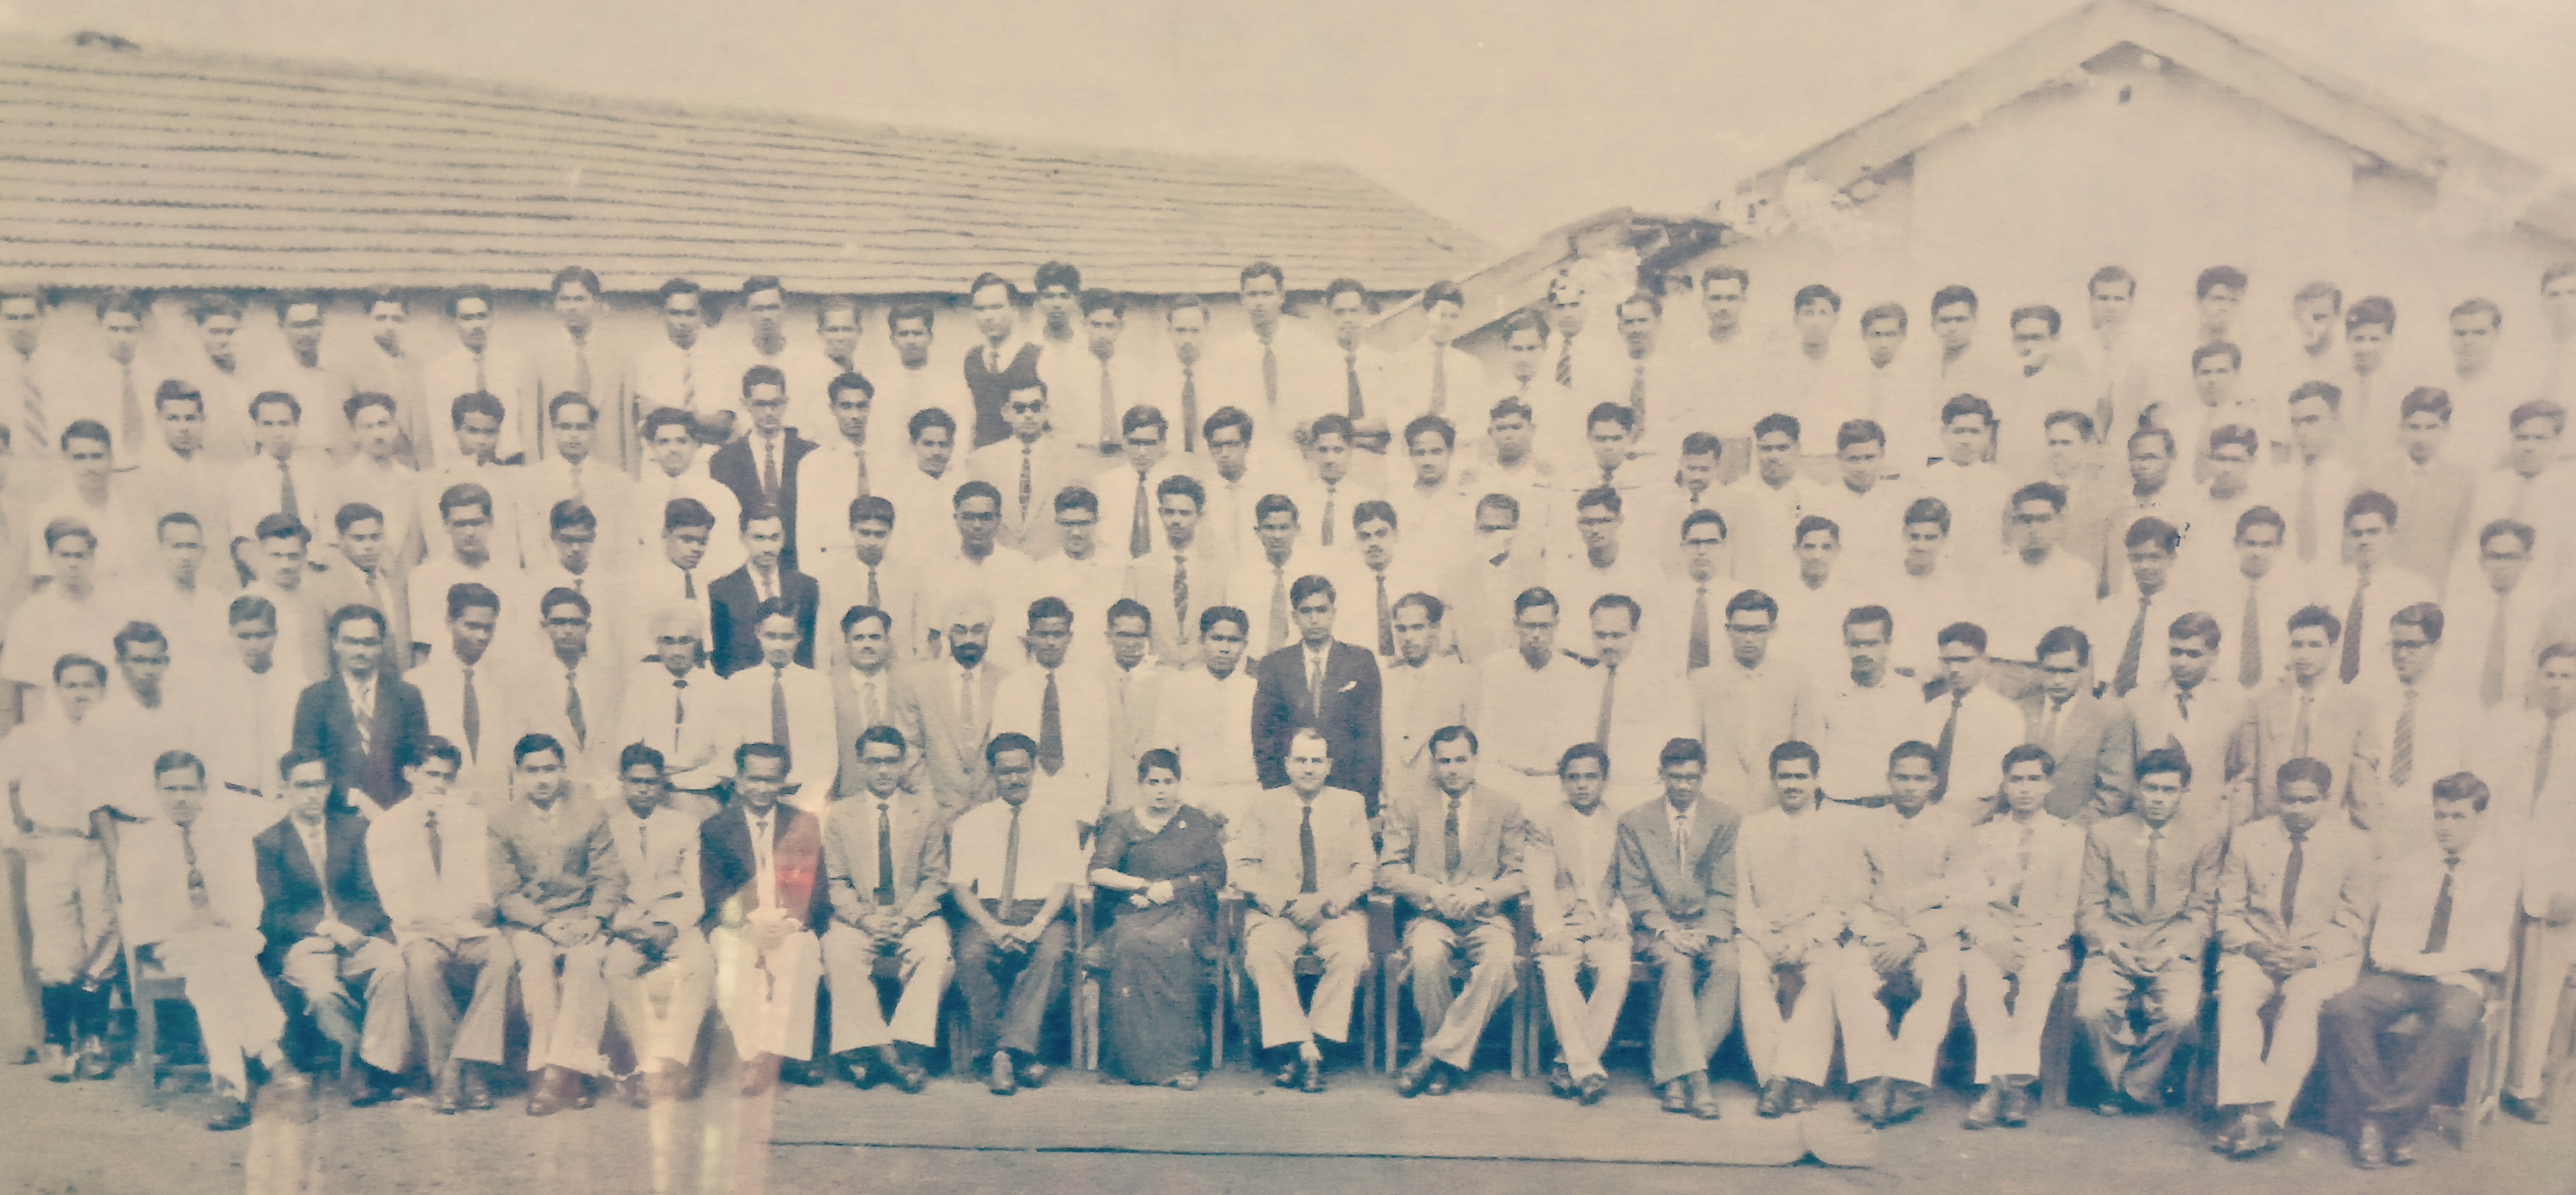
\includegraphics[width=1\textwidth]{images/new-images/06-Rajaji-TS.jpg}
\caption{\small{Training school students and the teachers. Col Ottley, the warden of the hostel is in the middle of the front row. I am standing in the fourth row, third after the person behind Col. Ottley.}}
\end{figure}

Most of the teachers were excellent. We voted KK Gupta as the best teacher.
In our batch there were 50 + 50 + 50 trainees, in Physics, Chemistry
and Engineering. There were no girls! Over the years, all this has changed.\
There were many South Indians\break among us. We used to come to the hostel 
mess in dhoties.\break Ramanna passed an order disallowing dhoties. We went on 
a hunger strike. It ended after a day; we capitulated after a day of 
starvation!
\vskip 1pt
I got first rank at the end of the training. For that I received the 
Homi Bhabha Gold medal from Prime Minister Manmohan Singh during the 
Golden Jubilee celebration of the Training\break School in 2007. But that was 
the second award for the same thing! Since I got not only first rank but 
my marks were way above those of the nearest to me, Colonel Ottley the 
hostel\break warden gifted me a book: ``The man in the grey flannel suit". It 
was filmed in Hollywood with the famous actor Gregory Peck.
 
I got freedom to choose between TIFR and AEET for my\break research. All the 
trainees who were above a certain rank were\break allowed to choose BARC 
(called AEET at that time) or TIFR. I\break chose TIFR.
\smallskip

\begin{figure}[H]
\centering
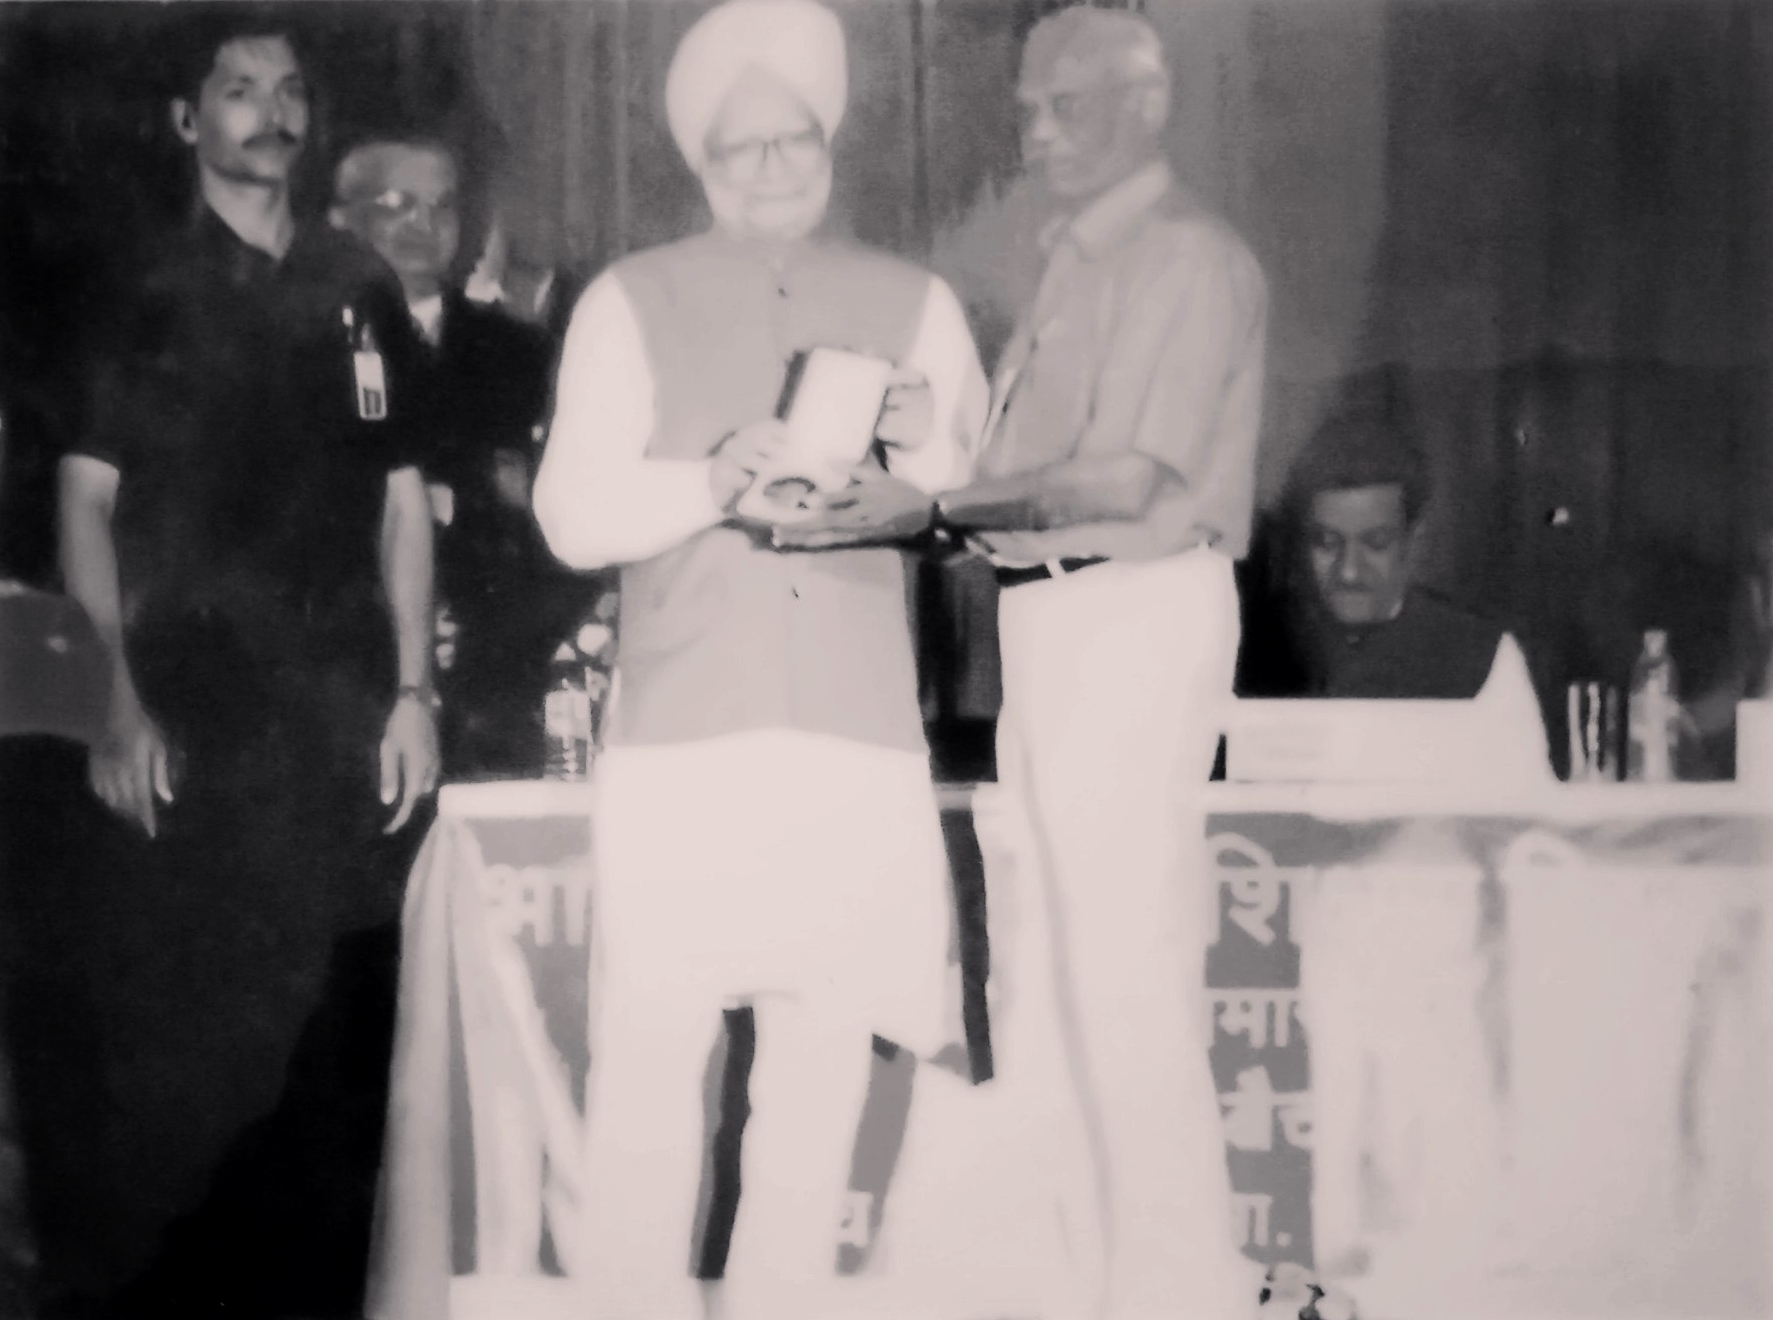
\includegraphics[width=0.9\textwidth]{images/Rajaji-04.jpg}
\caption{\small{Prime Minister Manmohan Singh presenting the Homi Bhabha
gold medal, 2007.}}
\end{figure}

